%%%%%%%%%%%%%%%%%%%%%%%%%%%%%%%%%%%%%%%%%
% KOMA-Script Presentation
% LaTeX Template
% Version 1.1 (18/10/15)
%
% This template has been downloaded from:
% http://www.LaTeXTemplates.com
%
% Original Authors:
% Marius Hofert (marius.hofert@math.ethz.ch)
% Markus Kohm (komascript@gmx.info)
% Described in the PracTeX Journal, 2010, No. 2
%
% License:
% CC BY-NC-SA 3.0 (http://creativecommons.org/licenses/by-nc-sa/3.0/)
%
%%%%%%%%%%%%%%%%%%%%%%%%%%%%%%%%%%%%%%%%%

%----------------------------------------------------------------------------------------
%	PACKAGES AND OTHER DOCUMENT CONFIGURATIONS
%----------------------------------------------------------------------------------------
% KOMA-Script_MDPI_jpm-1309345
% compiling only on TexLive 2019

\documentclass[
paper=landscape,
paper=160mm:90mm, %128mm:96mm, % The same paper size as used in the beamer class
fontsize=11pt, % Font size
pagesize, % Write page size to dvi or pdf
parskip=half-, % Paragraphs separated by half a line
]{scrartcl} % KOMA script (article)

\linespread{1.12} % Increase line spacing for readability



%~~~~~~~~~~~~~~~~~~~~~~~~~~~~~~~~~~~~~~~~~~~~~~~
% from main.tex
%%%%%%%%%%%%%%%%%%%%%%%%%%%%%%%%%% Tex
\maxdeadcycles=1000 % Output loop---200 consecutive dead cycles.

\usepackage{todonotes}

\usepackage{floatrow} % for side caption (beside)
%\floatsetup[widefigure]{margins=hangleft,capposition=beside,capbesideposition={center,outside},floatwidth=\textwidth} % {center,outside}
\usepackage{amsmath,amsfonts}
\usepackage{tikz-imagelabels} % for  tikz
%\usepackage[]{caption} % bf
%\newcommand{\bcaption}[2]{\caption{\textbf{#1} #2}}
%\usepackage{outlines}
% mark in blue or red
%\usepackage{xcolor}

%\usepackage{xr-hyper}
\usepackage{hyperref}
%\newcommand{\R}[1]{\label{#1}\linelabel{#1}} % for \label page and line
%\newcommand{\R}[1]{\linelabel{#1}} % for \label page and line
%\newcommand{\lr}[1]{page~\pageref{#1} (line~\lineref{#1})} % for \ref page and line
% for xr in your preamble
% https://www.overleaf.com/learn/how-to/Cross_referencing_with_the_xr_package_in_Overleaf
%\makeatletter
%\newcommand*{\addFileDependency}[1]{% argument=file name and extension
%  \typeout{(#1)}
%  \@addtofilelist{#1}
%  \IfFileExists{#1}{}{\typeout{No file #1.}}
%}
%\makeatother

%\newcommand*{\myexternaldocument}[1]{%
%    \externaldocument{#1}%
%    \addFileDependency{#1.tex}%
%    \addFileDependency{#1.aux}%
%}
% my external document I would like to reference the labels of. 
%\myexternaldocument{Supplementary_figures} %.tex .aux

\usepackage{array}
\usepackage{ragged2e}
\usepackage{rotating}
\usepackage{tabularx} % for resizebox?
\usepackage{makecell}
% \usepackage{array}
\usepackage{multirow}
\usepackage{colortbl}
\usepackage{hhline}
\usepackage{siunitx} % for  1e-10 scientific notation
%\usepackage{caption}
%\usepackage{subcaption}
%\usepackage{subcaption} % for figure  side by side, subfigure

%DIF 140a141
\usepackage{pbox} %DIF > 
%DIF -------

\usepackage{booktabs, multirow} % for borders and merged ranges
\usepackage{soul}% for underlines
%\usepackage[table]{xcolor} % for cell colors
\usepackage{changepage,threeparttable} 

%%% for abbreviations, or acronyms
\usepackage[acronym, nopostdot]{glossaries}  % automake
\usepackage{glossary-inline}
%\setacronymstyle{long-short}
%\renewcommand*{\glossarysection}[2][]{} 
%\renewcommand*{\glossarysection}[2][]{\textbf{#1}: }
% for abbreviations environment
%\newcommand{\abbrlabel}[1]{\makebox[3cm][l]{\textbf{#1}\ \dotfill}}
\newenvironment{abbreviation}


%\section{abbreviation}
%%%%%%%%%%%%% Define abbreviation
%\makeglossaries %https://tex.stackexchange.com/questions/110095/list-of-acronyms-is-not-displayed



\newacronym{ncbi}{NCBI}{National Center for Biotechnology Information}
\newacronym{degs}{DEGs}{differentially expressed genes}

\newacronym{ihc}{IHC}{immunohistochemistry}
\newacronym{fdr}{FDR}{false discovery rate}

\newacronym{hpa}{HPA}{the Human Protein Atlas}
\newacronym{hnscc}{HNSCC}{head and neck squamous cell carcinoma}
\newacronym{tcga}{TCGA}{the Cancer Genome Atlas}
\newacronym{tcpa}{TCPA}{the Cancer Proteome Atlas}
\newacronym{rna}{RNA}{ribonucleic acid}
\newacronym{rnaseq}{RNA-Seq}{RNA sequencing}
\newacronym{lncrna}{lncRNA}{long non-coding RNA}
%\newacronym{km}{KM}{Kaplan--Meier}
\newacronym{rppa}{RPPAs}{reverse-phase protein arrays}
\newacronym{rpma}{RPMA}{reverse-phase protein lysate microarray}

\newacronym{mmp}{MMP}{matrix metalloproteinase}
 %DKK1, CAMK2N1, STC2, PGK1, SURF4, USP10, NDFIP1, FOXA2, STIP1, and DKC1
 %ZNF557, ZNF266, IL19, MYO1H, FCGBP, LOC148709, EVPLL, PNMA5, KIAA1683, and NPB

\newacronym{DKK1}{DKK1}{dickkopf WNT signaling pathway inhibitor 1} 
\newacronym{CAMK2N1}{CAMK2N1}{calcium/calmodulin dependent protein kinase II inhibitor 1} 
\newacronym{CALML5}{CALML5}{calmodulin like 5}

\newacronym{STC2}{STC2}{stanniocalcin 2} 
\newacronym{PGK1}{PGK1}{phosphoglycerate kinase 1} 
\newacronym{SURF4}{SURF4}{surfeit 4} 
\newacronym{USP10}{USP10}{ubiquitin specific peptidase 10} 
\newacronym{NEDD4}{NEDD4}{neural precursor cell expressed, developmentally down-regulated 4}
\newacronym{NDFIP1}{NDFIP1}{NEDD4 family interacting protein 1} 
\newacronym{FOXA2}{FOXA2}{forkhead box A2} 
\newacronym{STIP1}{STIP1}{stress-induced-phosphoprotein 1} 
\newacronym{DKC1}{DKC1}{dyskeratosis congenita 1, dyskerin} 

\newacronym{ZNF557}{ZNF557}{zinc finger protein 557} 
\newacronym{ZNF266}{ZNF266}{zinc finger protein 266} 
\newacronym{IL19}{IL19}{interleukin 19} 
\newacronym{MYO1H}{MYO1H}{myosin 1H} 
\newacronym{FCGBP}{FCGBP}{Fc fragment of IgG binding protein} 
\newacronym{LOC148709}{LOC148709}{LncRNA LOC148709} 
\newacronym{EVPLL}{EVPLL}{envoplakin-like protein} 
\newacronym{PNMA5}{PNMA5}{paraneoplastic antigen like 5} 
%\newacronym{KIAA1683}{KIAA1683}{IQCN, IQ Motif Containing N} 
\newacronym{IQCN}{IQCN}{IQ motif containing N} % previous name KIAA1683
% "IQ'' refers to the first two amino acids of the motif: isoleucine (commonly) and glutamine (invariably)
\newacronym{NPB}{NPB}{neuropeptide B} 

 \newacronym{rt}{RT}{radiation therapy}
 \newacronym{nccn}{NCCN}{National Comprehensive Cancer Network}
 \newacronym{hif}{HIF}{hypoxia-inducible factor}
 \newacronym{egfr}{EGFR}{epidermal growth factor receptor}
 \newacronym{ras}{RAS}{rat sarcoma}
 \newacronym{hras}{HRAS}{Harvey rat sarcoma viral oncoprotein}
 \newacronym{erk}{ERK}{extracellular signal-regulated kinases}
 \newacronym{us}{US}{United States}
 \newacronym{fda}{FDA}{Food and Drug Administration}
 \newacronym{tpf}{Tax-PF}{docetaxel, cisplatin, and 5-fluorouracil}
 \newacronym{tki}{TKI}{tyrosine kinase inhibitor}
 \newacronym{her}{HER}{human epidermal growth factor receptor}
 \newacronym{ici}{ICI}{immune-checkpoint inhibitor}
 \newacronym{ctla4}{CTLA-4}{cytotoxic T lymphocyte antigen 4}
 \newacronym{pd1}{PD-1}{programmed death 1}
 \newacronym{pdl1}{PD-L1}{programmed death ligand 1}
 \newacronym{tim3}{TIM-3}{T-cell immunoglobulin mucin protein 3}
 \newacronym{lag3}{LAG-3}{lymphocyte activation gene 3}
 \newacronym{ifng}{IFN-$\gamma$}{interferon gamma}
 \newacronym{tigit}{TIGIT}{T cell immunoglobin and immunoreceptor tyrosine-based inhibitory motif}
 \newacronym{gitr}{GITR}{glucocorticoid-induced tumor necrosis factor receptor}
 \newacronym{vista}{VISTA}{V-domain Ig suppressor of T-cell activation}
 \newacronym{tmsb4x}{TMSB4X}{thymosin beta-4 X-linked}
 \newacronym{emt}{EMT}{epithelial-mesenchymal-transition}
 \newacronym{gdc}{GDC}{Genomic Data Commons}
 \newacronym{nci}{NCI}{the National Cancer Institute}
 \newacronym{gdac}{GDAC}{genome data analysis center}
 \newacronym{rest}{REST}{Representational State Transfer} 
 \newacronym{api}{API}{application programmable interface}
\newacronym{grch38}{GRCh38}{Genome Reference Consortium Homo sapiens genome assembly 38}
\newacronym{fpkm}{FPKM}{Fragments per kilobase per million reads mapped}
\newacronym{rsem}{RSEM}{RNA-Seq by Expectation-Maximization}
\newacronym{slca}{SLC35E2A}{solute carrier family 35 member E2A}
\newacronym{slcb}{SLC35E2B}{solute carrier family 35 member E2B}
\newacronym{cde}{CDE}{Common Data Element}
\newacronym{id}{ID}{identification}
\newacronym{ajcc}{AJCC}{the American Joint Committee on Cancer}
\newacronym{uicc}{UICC}{he Union for International Cancer Control}
\newacronym{tnm}{TNM}{the tumor size (T), cervical lymph node metastases (N), and distal metastasis status (M)}
\newacronym{ci95}{95\% CI}{95\% confidence interval}
\newacronym{os}{OS}{overall survival}
\newacronym{hr}{HR}{hazard ratio}
\newacronym{hpv}{HPV}{human papillomavirus}
\newacronym{ene}{ENE}{extra-nodal extension}
\newacronym{lvsi}{LVSI}{lymph-vascular space invasion}
\newacronym{pni}{PNI}{perineural invasion}
\newacronym{doi}{DOI}{depth of invasion}
\newacronym{lnd}{LND}{lymph node density}
\newacronym{wpoi5}{WPOI-5}{worst pattern of invasion score 5}
\newacronym{glut4}{GLUT4}{glucose transporter 4}
\newacronym{slc2a4}{SLC2A4}{solute carrier family 2 member A4}
\newacronym{trim24}{TRIM24}{tripartite motif-containing 24}
\newacronym{til}{TIL}{tumor-infiltrating lymphocytes}
\newacronym{tmb}{TMB}{tumor mutational burden}




%------------------------------------------------
\usepackage{outlines}
\usepackage[font={small}]{caption}
\newcommand{\bcaption}[2]{\caption{\textbf{#1} #2}}


\usepackage[margincaption]{sidecap}

\usepackage{subcaption} % for figure  side by side, subfigure

%%%%%% updated 2020 by esdd
%% https://tex.stackexchange.com/questions/547723/latex-throws-errors-on-section
%------------------------------------------------
% Colors
\usepackage[]{xcolor}  % table % Required for custom colors
% Define a few colors for making text stand out within the presentation
\definecolor{mygreen}{RGB}{44,85,17}
\definecolor{myblue}{RGB}{34,31,217}
\definecolor{mybrown}{RGB}{194,164,113}
\definecolor{myred}{RGB}{255,66,56}
% Use these colors within the presentation by enclosing text in the commands below

\newcommand*{\mygreen}[1]{\textcolor{mygreen}{#1}}
\newcommand*{\myblue}[1]{\textcolor{myblue}{#1}}
\newcommand*{\mybrown}[1]{\textcolor{mybrown}{#1}}
\newcommand*{\myred}[1]{\textcolor{myred}{#1}}

\definecolor{asparagus}{rgb}{0.53, 0.66, 0.42}

\newenvironment{MyColorPar}[1]{% for RED marked of revision
    \leavevmode\color{#1}\ignorespaces%
}{%
}%


% Margins
\usepackage[ % Page margins settings
  includeheadfoot,
  top=-1mm,
  bottom=1.5mm,
  left=1mm,
  right=3.5mm,
  headsep=0mm,
  footskip=8.5mm
]{geometry}

% Fonts
\usepackage[T1]{fontenc}     % For correct hyphenation and T1 encoding
\usepackage{lmodern} % Default font: latin modern font
%\usepackage{fourier} % Alternative font: utopia
%\usepackage{charter} % Alternative font: low-resolution roman font
\renewcommand{\familydefault}{\sfdefault} % Sans serif - this may need to be commented to see the alternative fonts

% Various required packages
\usepackage{amsthm} % Required for theorem environments
\usepackage{bm} % Required for bold math symbols (used in the footer of the slides)
\usepackage{tikz} % Required for colored boxes, loads graphicx and other packages
\usepackage{booktabs} % Required for horizontal rules in tables
\usepackage{multicol} % Required for creating multiple columns in slides
\usepackage{lastpage} % For printing the total number of pages at the bottom of each slide

\usepackage{microtype} % Better typography

% Slide layout configuration
\usepackage[automark]{scrlayer-scrpage} % Required for customization of the header and footer
\clearpairofpagestyles % Remove the default header and footer
\AddLayersAtBeginOfPageStyle{scrheadings}{headerbg,footerbg}% add background layers
\setkomafont{pageheadfoot}{\normalfont\sffamily} % Font settings for the header and footer
\setkomafont{pagehead}{\color{white}}
% Header configuration - if you don't want a header remove this block
\DeclareNewLayer[
  background,
  head,
  hoffset=0pt,
  width=\paperwidth,
  mode=picture,
  contents=\putLL{\myblue{\rule{\layerwidth}{\layerheight}}}
]{headerbg}

\ihead{\rightbotmark}

% Footer configuration
\KOMAoptions{footwidth=\textwidth+2mm:0pt}
\setkomafont{pagefoot}{\color{black}\tiny} % Small font size for the footnote
%\DeclareNewLayer[
  %background,
  %foot,
  %hoffset=0pt,
  %width=\paperwidth,
  %mode=picture,
  %contents=\putLL{\myblue{\rule{\layerwidth}{\layerheight}}}
%]{footerbg}
\ifoot{\myauthor\ \raisebox{0.2mm}{$\bm{\vert}$}\ \myuni} % Left side text
\ofoot*{\pagemark/\pageref{LastPage}} % Right side

% Sets vertical centering of slide contents with increased space between paragraphs/lists
\makeatletter
\renewcommand*{\@textbottom}{\vskip \z@ \@plus 1fil}
\newcommand*{\@texttop}{\vskip \z@ \@plus .5fil}
\setparsizes{1em}{\z@\@plus .25fil}{0pt plus 1fil}
\makeatother

% Remove page numbers and the dots leading to them from the outline slide
\DeclareTOCStyleEntries[linefill=\hfill,pagenumberbox=\gobble]{section}{section,subsection,subsubsection}
%\newcommand*\gobble[1]{}
\AfterTOCHead{\small}

%\renewcaptionname{english}{\contentsname}{Outline} % contentsname % Change the name of the table of contents
% Section spacing - deeper section titles are given less space due to lesser importance
\RedeclareSectionCommands[beforeskip=0pt,afterskip=0pt,afterindent=true,runin=false]{section,subsection,subsubsection}
\RedeclareSectionCommand[afterskip=-1mm]{subsection}
\RedeclareSectionCommand[afterskip=-2mm]{subsubsection}
\setcounter{secnumdepth}{\partnumdepth} % How deep sections are numbered

% Theorem style
\newtheoremstyle{mythmstyle} % Defines a new theorem style used in this template
  {0.5em} % Space above
  {0.5em} % Space below
  {} % Body font
  {} % Indent amount
  {\sffamily\bfseries} % Head font
  {} % Punctuation after head
  {\newline} % Space after head
  {\thmname{#1}\ \thmnote{(#3)}} % Head spec

\theoremstyle{mythmstyle} % Change the default style of the theorem to the one defined above
\newtheorem{theorem}{Theorem}[section] % Label for theorems
\newtheorem{remark}[theorem]{Remark} % Label for remarks
\newtheorem{algorithm}[theorem]{Algorithm} % Label for algorithms


% The code for the box which can be used to highlight an element of a slide (such as a theorem)
\newcommand*{\mybox}[2]{% The box takes two arguments: width and content
  \par\noindent
  \begin{tikzpicture}[mynodestyle/.style={rectangle,draw=myblue,thick,inner sep=2mm,text justified,top color=white,bottom color=white,above}]
    \node[mynodestyle,at={(0.5*#1+2mm+0.4pt,0)}]{% Box formatting
      \begin{minipage}[t]{#1}
      #2
      \end{minipage}%
    };
  \end{tikzpicture}
\par\vspace{-1.3em}}

%----------------------------------------------------------------------------------------
%	PRESENTER INFORMATION
%----------------------------------------------------------------------------------------

\newcommand*{\mytitle}{Transcriptomic Analysis for Prognostic Value in Head and Neck Squamous Cell Carcinoma} % Title
\newcommand*{\runninghead}{HNSCC Biomarker} % Running head displayed on almost all slides
\newcommand*{\myauthor}{Tex Li-Hsing Chi} % Presenters name(s)
\newcommand*{\mydate}{\today} % Presentation date
\newcommand*{\myuni}{Taipei Medical University} % University or department

%----------------------------------------------------------------------------------------

\begin{document}

%----------------------------------------------------------------------------------------
%	TITLE SLIDE
%----------------------------------------------------------------------------------------

% Title slide - you may have to tweak a few of the numbers if you wish to make changes to the layout
\thispagestyle{empty} % No slide header and footer
\begin{tikzpicture}[remember picture,overlay] % Background box
  \node [xshift=\paperwidth/2,yshift=\paperheight/2] at (current page.south west)
    [rectangle,fill,inner sep=0pt,minimum width=\paperwidth,minimum height=\paperheight/2.1,top color=myblue,bottom color=myblue]{}; % Change the height of the box, its colors and position on the page here
\end{tikzpicture}
% Text within the box
\begin{flushright}
  \vspace{1.6cm}
  \color{white}\sffamily
  {\bfseries\Large\mytitle\par}% Title
  \vspace{0.5cm}
  \normalsize
  \myauthor\par % Author name
  \mydate\par % Date
  \myuni\par
  \vfill
\end{flushright}

\clearpage
%----------------------------------------------------------------------------------------
%	TABLE OF CONTENTS
%----------------------------------------------------------------------------------------

\thispagestyle{empty} % No slide header and footer

\small\tableofcontents % Change the font size and print the table of contents - it may be useful to shrink the font size further if the presentation is full of sections
% To exclude sections/subsections from the table of contents, put an asterisk after \(sub)section like so: \section*{Section Name}

\clearpage

%----------------------------------------------------------------------------------------
%	PRESENTATION SLIDES
%----------------------------------------------------------------------------------------

%\section*{Vize}

%\clearpage

%------------------------------------------------



%------------------------------------------------


\section*{Verbatim}

How to include a theorem in this presentation:
\begin{verbatim}
\mybox{0.8\textwidth}{
\begin{theorem}[Murphy (1949)]
Anything that can go wrong, will go wrong.
\end{theorem}
}
\end{verbatim}

\clearpage

%------------------------------------------------



\subsection*{Figure}

%\clearfloatsetup{figure}
%\floatsetup[figure]{style=no,capposition=beside,capbesideposition={center,inside},capbesideframe=yes,facing=yes}

\begin{figure}[ht]
\floatbox[{\capbeside\thisfloatsetup{capbesideposition={right,center},capbesidewidth=.35\linewidth,capbesidesep=quad}}]{figure}[\FBwidth]
{\caption{\texttt{capbesidesep=quad}. I want to thank Sonia. The caption can contain any text but needs to describe the image with enough detail for a reader to completely understand the image.}}
{
\includegraphics[width=0.6\textwidth]{placeholder.jpg}}
\end{figure}
%
\includegraphics[width=9cm]{placeholder}

%\sidecaptionvpos{c}
%\caption{I want to thank Sonia.}
%\end{captionbeside}


\clearpage

%------------------------------------------------



\section{Introduction0}


\begin{outline}

\1 Aliquam blandit faucibus nisi, sit amet dapibus enim tempus eu

\2 Nulla commodo, erat quis gravida posuere
\1 elit lacus lobortis est, quis porttitor odio mauris at libero
\1 Nam cursus est eget velit posuere pellentesque
\1 Vestibulum faucibus velit a augue condimentum quis convallis nulla gravida

\end{outline}


\clearpage


% figure replaced by minipage
%\clearfloatsetup{figure}
%\floatsetup[figure]{style=no,capposition=beside,capbesideposition={center,outside},capbesideframe=yes,facing=yes}

\todo{python code for all figures}

\begin{figure}[ht]
\floatbox[{\capbeside\thisfloatsetup{capbesideposition={right,center},capbesidewidth=.35\linewidth,capbesidesep=quad}}]{figure}[\FBwidth]
%\centering
%\widefigure, keepaspectratio
{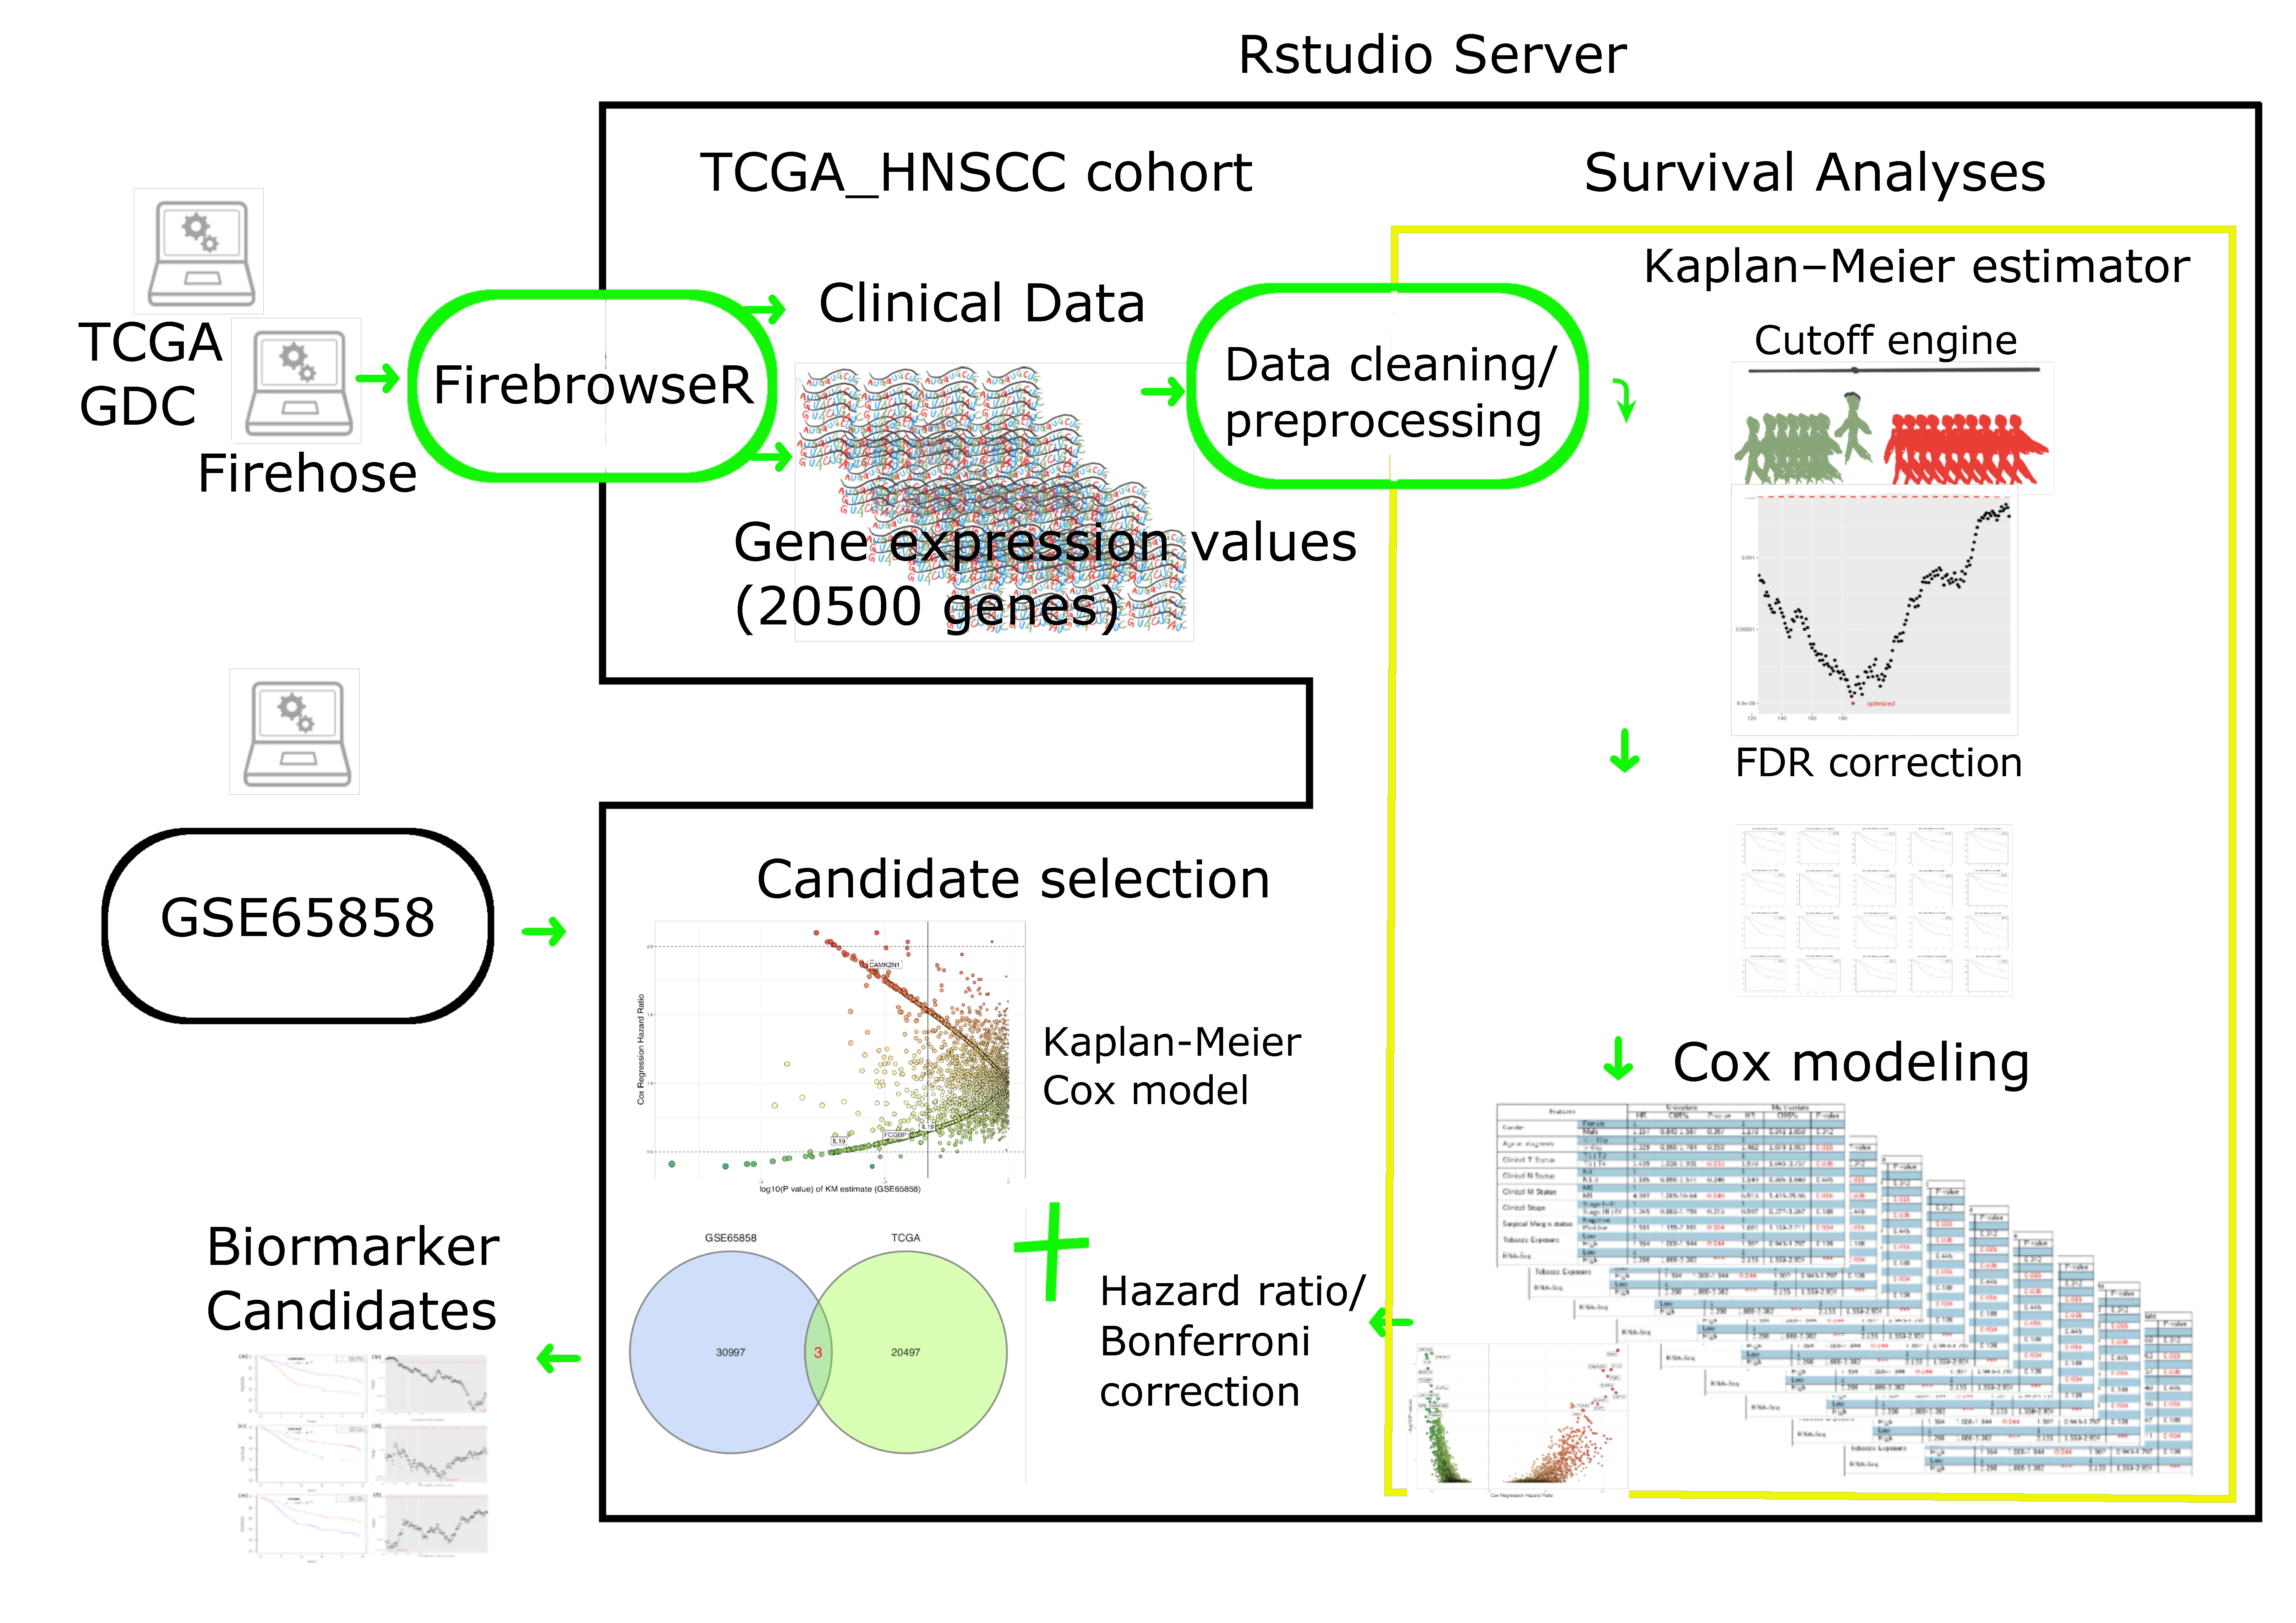
\includegraphics[width=7cm]{Figure_1_manuscript_workflow.pdf}} % .PDF is better than .png
%, height=8cm
%\caption % , step 1 (\textcolor{blue}{blue line}: main procedure) and step 2 (\textcolor{orange}{orange line}: analysis export).
%Step 3 (purple line: dealing with surgical margin).
%\sidecaptionvpos{c}
{\caption{\hl{A workflow of \acrshort{hnscc} biomarker discovery.}
The workflow includes data retrieval from the TCGA GDC data portal, data processing with merging and cleaning, and then performing the survival analyses (within \textcolor{yellow}{yellow} square).}} %The Cutoff engine (in R script: cutofFinder\_func.HNSCC.R, a serial cutoff for grouping patients with \textcolor{asparagus}{low} or \textcolor{red}{high} expression of a specific gene, to yield a collection of \protect\textit{P} values; please see Materials and Methods section for details) might calculate all possible Kaplan--Meier \protect\textit{P} values (corrected by \acrlong{fdr}, FDR, method) to find the optimal cutoff value of gene expression for subsequent Cox modeling. The candidate selection performs (1) dissecting and selection of candidate genes with further Bonferroni adjusted \protect\textit{P} values and the hazard ratios of a Cox model, based on the results from the survival analyses; (2) survival analyses of the other HNSCC dataset (GSE65858) using Kaplan--Meier estimates (with FDR corrections) and Cox modeling.\\ The biomarker candidates were consensus results of TCGA and GSE65858. (HNSCC: head and neck squamous cell carcinoma; TCGA: the Cancer Genome Atlas; RNA-Seq: RNA sequencing; GDC: Genomic Data Commons.)} } % end of caption

% Description:1) FDR correction of Kaplan--Meier \protect\textit{P} values during Cutoff finding; and 2) Bonferroni correction of Kaplan--Meier \protect\textit{P} values after Cox modeling for candidate selection.

%\end{minipage}
\end{figure}

\clearpage
%%%%%%%%%%%%%%%%%
% automatic generation by jpm2KOMO-script.py
%% [2011/08/08]
%%%%%%%


\section{Introduction}

\begin{figure}[ht]

\floatbox[{\capbeside\thisfloatsetup{capbesideposition={right,center},capbesidewidth=.35\linewidth,capbesidesep=quad}}]{figure}[\FBwidth]
%\centering
%\widefigure
{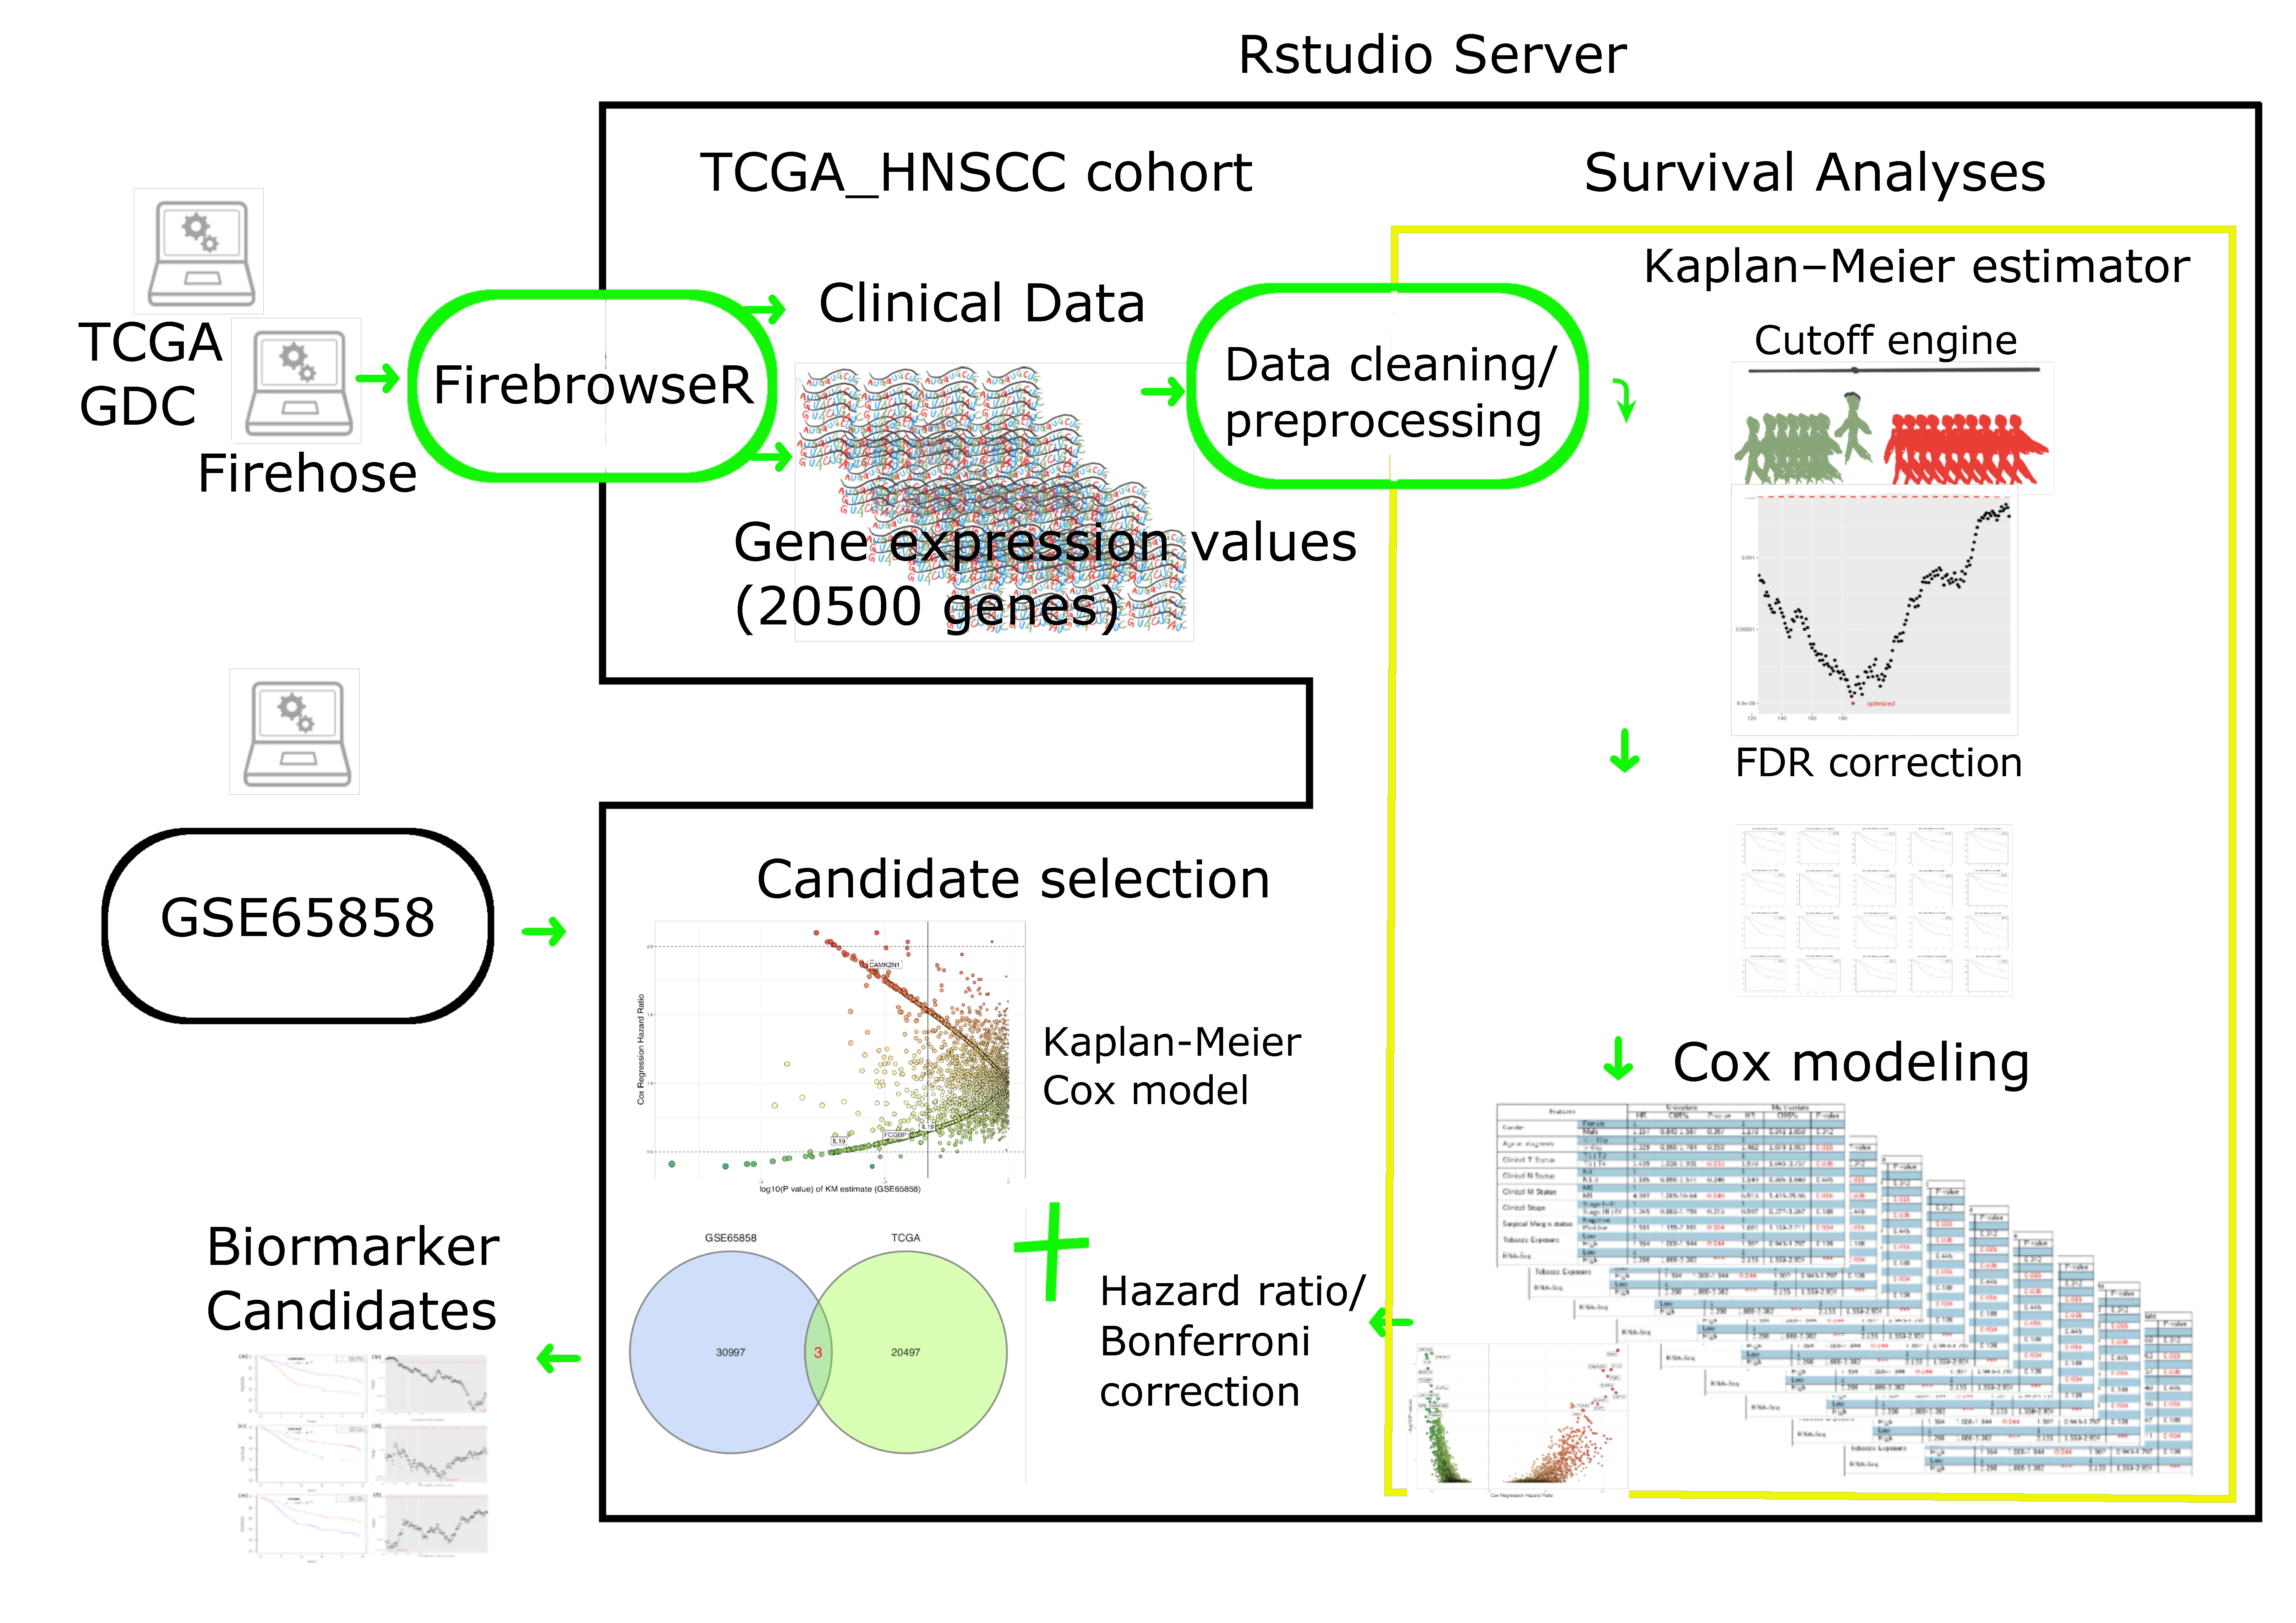
\includegraphics[width =\textwidth, height = 0.6\textheight, keepaspectratio]{Figure_1_manuscript_workflow} % .PDF is better than .png
} 
%, height=8cm
%\caption % , step 1 (\textcolor{blue}{blue line}: main procedure) and step 2 (\textcolor{orange}{orange line}: analysis export).
%Step 3 (purple line: dealing with surgical margin).
%MDPI: Picture is not clear. Please replace with a sharper image.
*** check *** {\caption{\hl{A workflow of} \acrshort{hnscc} biomarker discovery.} %MDPI: Is the bold necessary?
} 
{The workflow includes data retrieval from the TCGA GDC data portal, data processing with merging and cleaning, and then performing the survival analyses (within \textcolor{yellow}{yellow} square). The Cutoff engine (in R script: cutofFinder\_func.HNSCC.R, a serial cutoff for grouping patients with \textcolor{asparagus}{low} or \textcolor{red}{high} expression of a specific gene, to yield a collection of \protect\textit{p}~values; please see Materials and Methods section for details) might calculate all possible Kaplan--Meier \protect\textit{p}~values (corrected by \acrlong{fdr} (FDR) method) to find the optimal cutoff value of gene expression for subsequent Cox modeling.
The candidate selection performs (1) dissection and selection of candidate genes with further Bonferroni-adjusted \protect\textit{p}~values and the hazard ratios of a Cox model, based on the results from the survival analyses;
(2) survival analyses of the other HNSCC dataset (GSE65858) using Kaplan--Meier estimates (with FDR corrections) and Cox modeling. 
The biomarker candidates were consensus results of TCGA and GSE65858. 
%The selected genes were validated by third HNSCC cohort (GSE2837).\\
(HNSCC: head and neck squamous cell carcinoma; TCGA: the Cancer Genome Atlas; RNA-Seq: RNA sequencing; GDC: Genomic Data Commons.)}
%%%\label{fig:figure1}
% Description:1) FDR correction of Kaplan--Meier \protect\textit{p}~values during Cutoff finding; and 2) Bonferroni correction of Kaplan--Meier \protect\textit{p}~values after Cox modeling for candidate selection.


\end{figure}


\section{Results}



\begin{figure}[ht]
%\subsubsection{Figure 2:h}
%\begin{figure}[H]
%    \captionsetup[subfigure]{
%  font=footnotesize,
%  justification=raggedright
%  skip=10pt
%    }
%    \setlength{\abovecaptionskip}{35pt plus 3pt minus 2pt} % Chosen fairly arbitrarily
%\centering
\floatbox[{\capbeside\thisfloatsetup{capbesideposition={right,center},capbesidewidth=.35\linewidth,capbesidesep=quad}}]{figure}[\FBwidth]
%\centering
% not \widefigure
%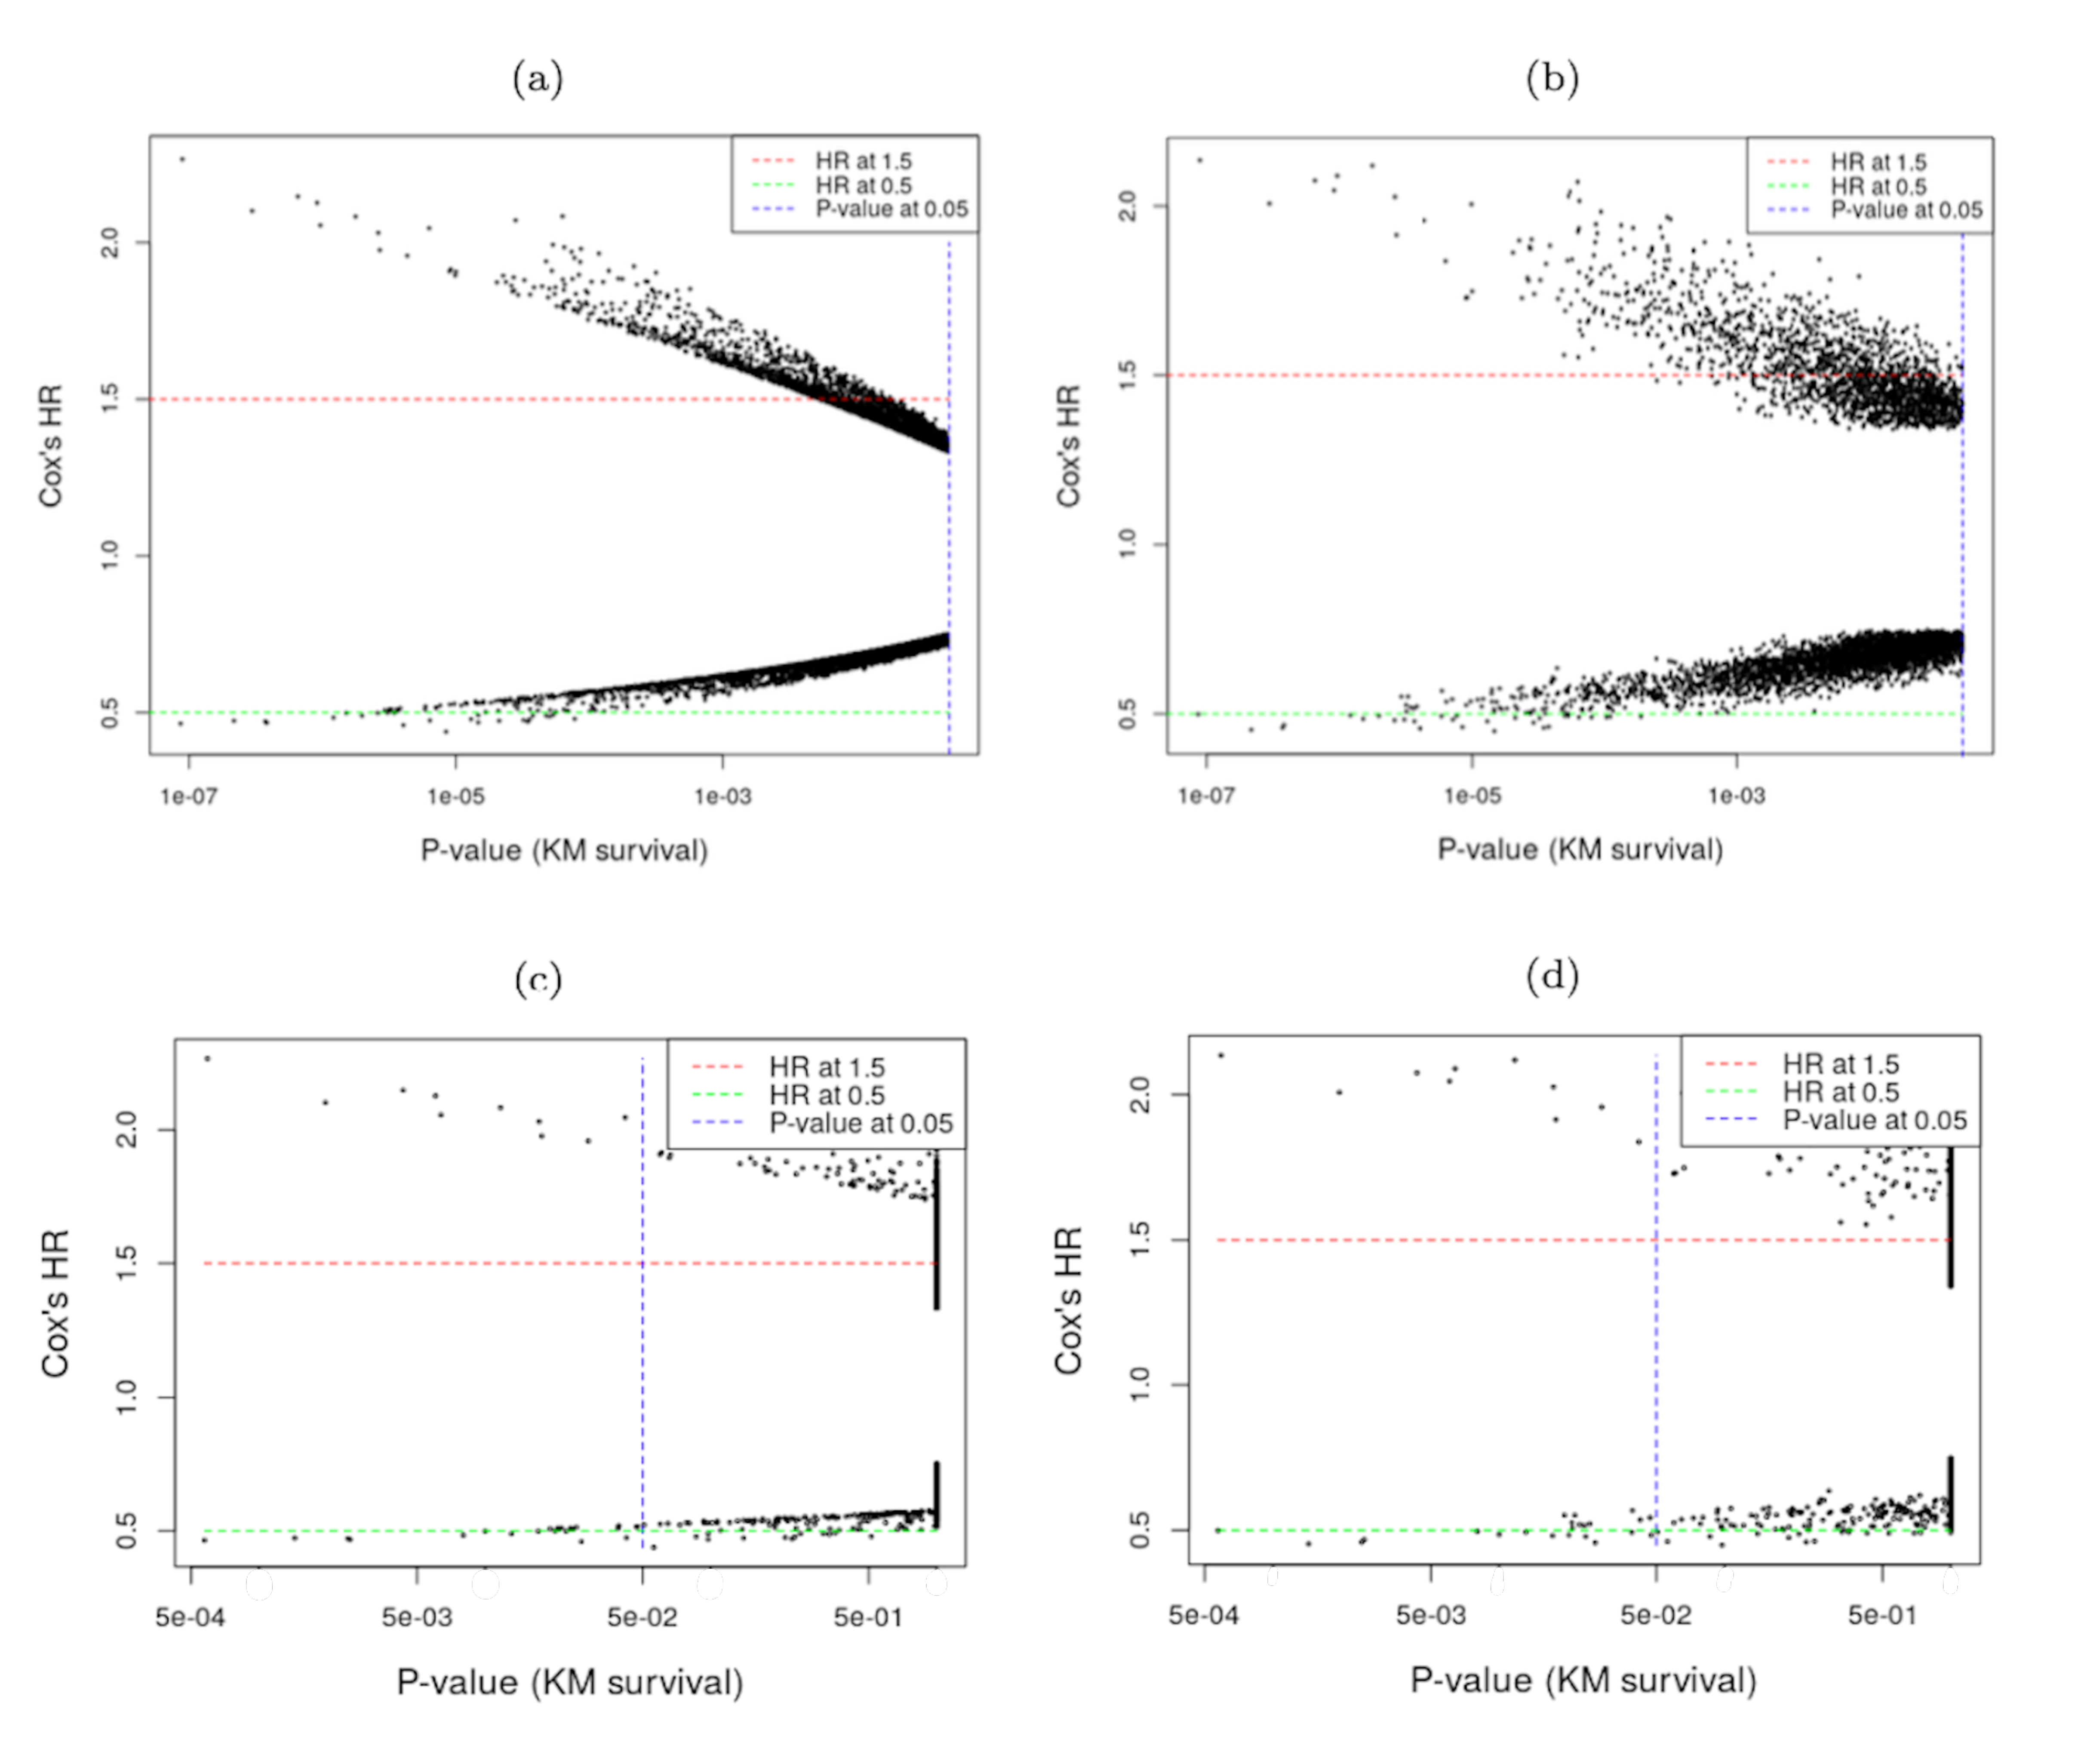
\includegraphics[width=14cm]{Figure2.pdf} %MDPI: Please revise the scientific notation format to a × 10b, and picture is not clear.ok
%\https://en.wikibooks.org/wiki/LaTeX/Floats,_Figures_and_Captions
% 2 by 2
% draw by tikz
{\setlength{\unitlength}{.78cm}
\begin{picture}(15, 1) %(1,0.55038404)%
\centering
%  \put(0,0){\includegraphics[width=14cm]{Figure_4_CAMK2N1_CALML5_FCGBP.pdf}}% X-axis: hyphen to minus sign
  \put(0.0, 1){\fontfamily{qcr}\selectfont
   (a)}%CAMK2N1
    \put(9.5, 1){\fontfamily{qcr}\selectfont
   (b)}%IL19 6.54e-06 -> CALML5 0.0001970348

\end{picture}

%% ab
    \begin{subfigure}[b]{0.35\textwidth}
%\subfloat[Subfigure 1 list of figures text][(a)]{
%        \vspace*{-5mm}
%        \caption{~}
%        \fbox{
        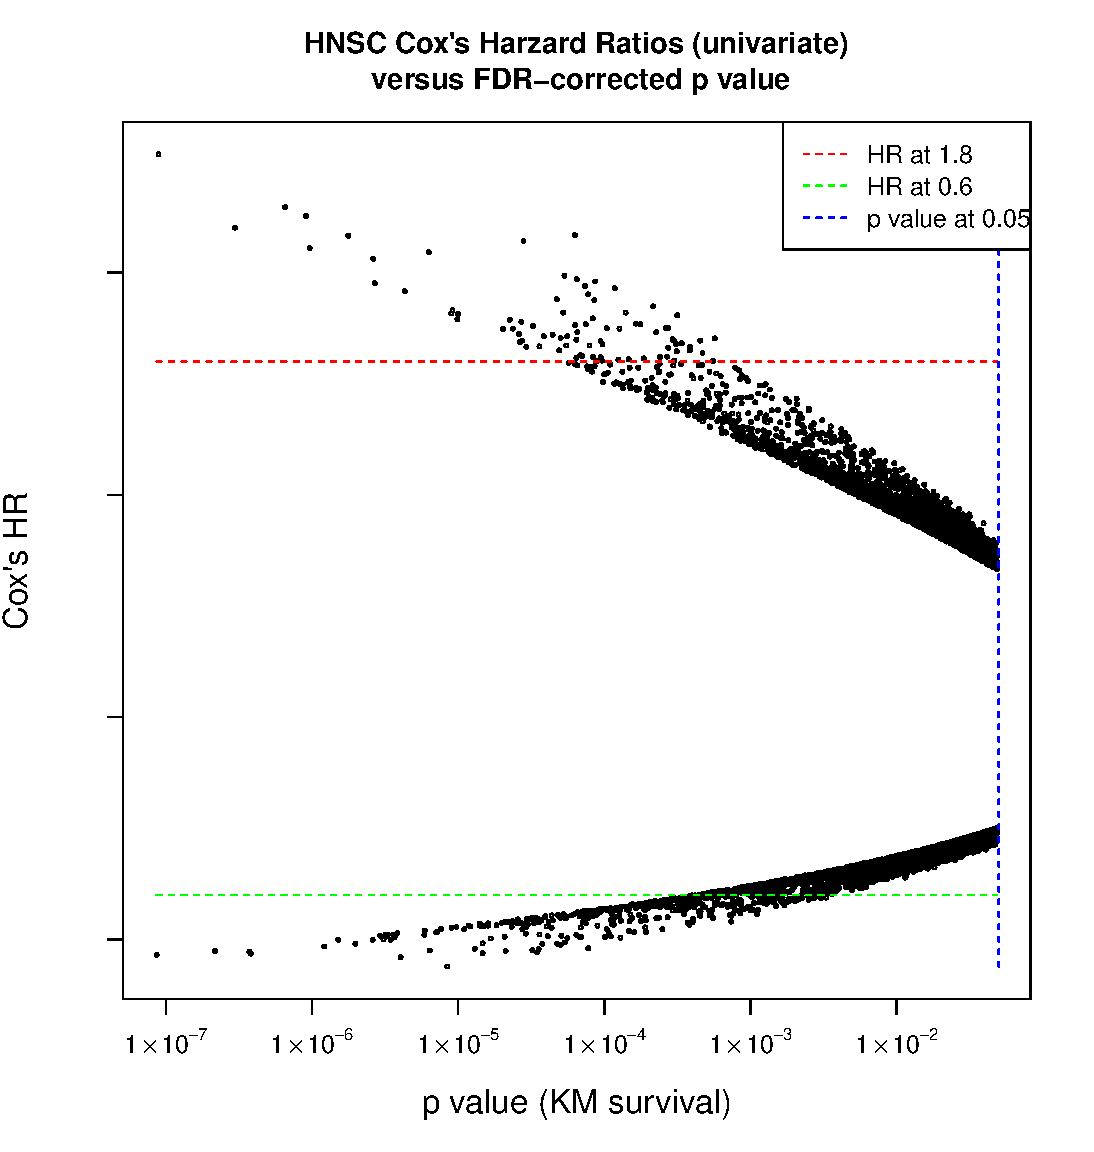
\includegraphics[width=1\textwidth]{Rplot02_FDRP_uniHR.pdf}  %}    %{Rplot02_rawP_uniHR.pdf}

    \end{subfigure} \hfill
%\subfloat[Subfigure 1 list of figures text][(b)]{
    \begin{subfigure}[b]{0.35\textwidth}
%        \caption{}
        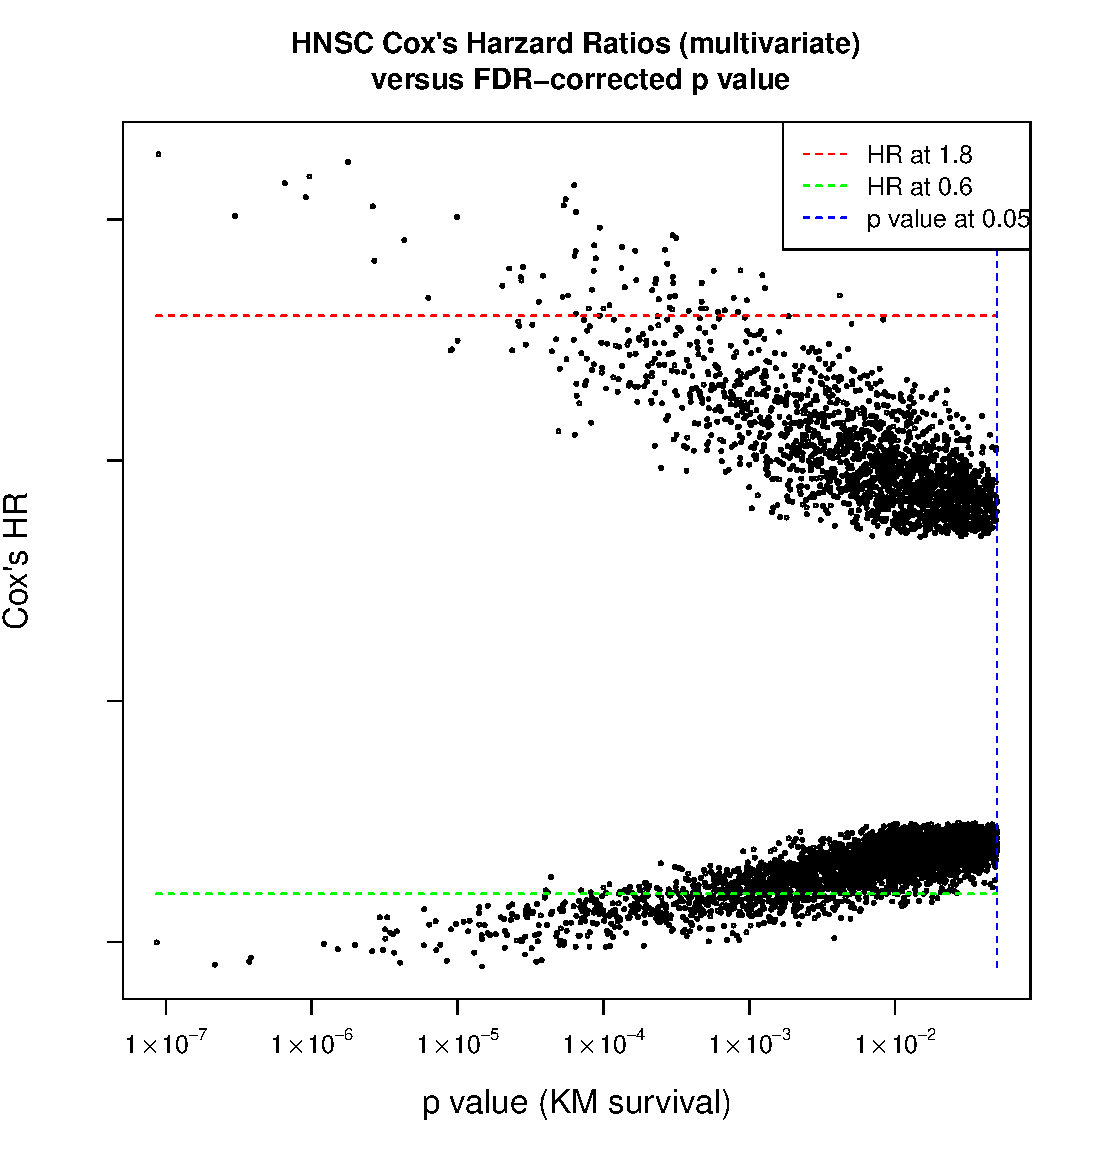
\includegraphics[width=6.5cm]{Rplot02_FDRP_multiHR.pdf}
%        \caption{}
    \end{subfigure} \\
%\end{adjustwidth}
%    \vskip\baselineskip

% ,clip,keepaspectratio, ,height=6.5cm
%\vspace{0.3cm}
% draw by tikz
\setlength{\unitlength}{.78cm}
\begin{picture}(15, 1) %(1,0.55038404)%
\centering
%  \put(0,0){\includegraphics[width=14cm]{Figure_4_CAMK2N1_CALML5_FCGBP.pdf}}% X-axis: hyphen to minus sign
  \put(0.0, 1){\fontfamily{qcr}\selectfont
   (c)}%CAMK2N1
    \put(9.5, 1){\fontfamily{qcr}\selectfont
   (d)}%IL19 6.54e-06 -> CALML5 0.0001970348

\end{picture}

%% cd
%\begin{adjustwidth}{-3em}{0em}
%\subfloat[Subfigure 1 list of figures text][(c)]{
    \begin{subfigure}[b]{0.25\textwidth}
%        \caption{}
        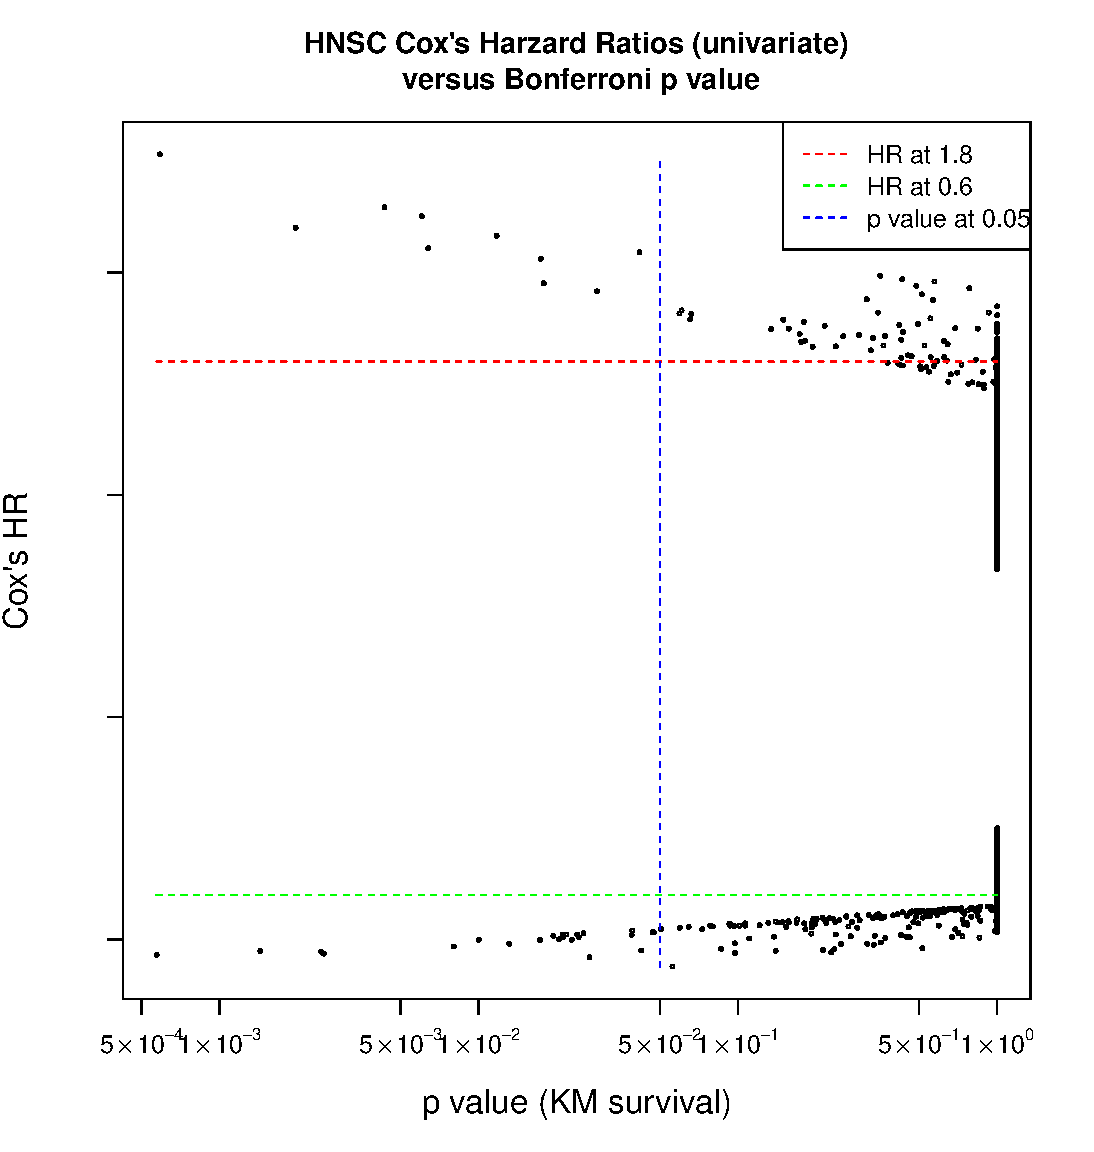
\includegraphics[width=6.5cm]{Rplot02_BonferroniP_uniHR.pdf}
%        \caption{}
    \end{subfigure} \hfill
%\qquad
%\subfloat[Subfigure 1 list of figures text][(d)]{
    \begin{subfigure}[b]{0.35\textwidth}
%        \caption{}
        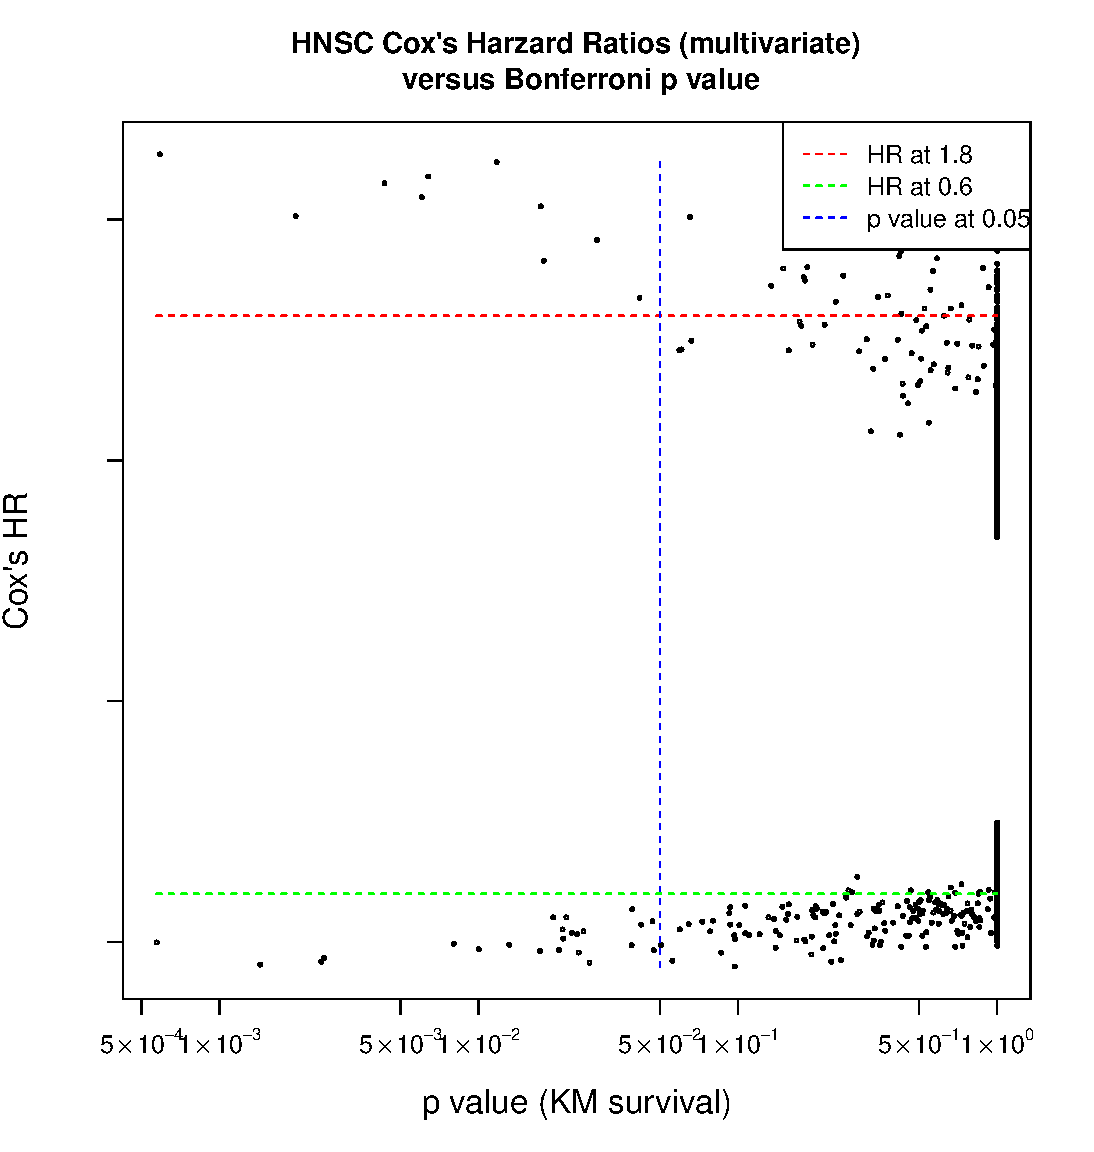
\includegraphics[width=6.5cm]{Rplot02_BonferroniP_multiHR.pdf}
%        \caption{}
    \end{subfigure}
} % end of {\includegraphics}

{\caption{The initial progress of candidate selection from the TCGA \acrshort{hnscc} cohort.
The \textit{p}~value of Kaplan--Meier survival was one of the selection criteria.
The effect size was estimated by Cox's hazard ratio.
Initial trial step: (\textbf{a}) univariate HR versus FDR-adjusted \textit{p}~value; (\textbf{b}) multivariate HR versus FDR-adjusted \textit{p}~value.
After stringent restriction by Bonferroni-adjusted \textit{p}~values and Cox's HR, a few top-ranked genes were acquired by
(\textbf{c}) univariate HR versus Bonferroni-adjusted \textit{p}~value;  (\textbf{d}) multivariate HR versus Bonferroni-adjusted \textit{p}~value.
(TCGA: \acrlong{tcga}; HR: hazard ratio; FDR: \acrlong{fdr}).}
}
%\label{fig:figure2}
\end{figure}% * = no overlapping with text


\begin{figure}[ht]

\floatbox[{\capbeside\thisfloatsetup{capbesideposition={right,center},capbesidewidth=.35\linewidth,capbesidesep=quad}}]{figure}[\FBwidth]
    %\centering
{    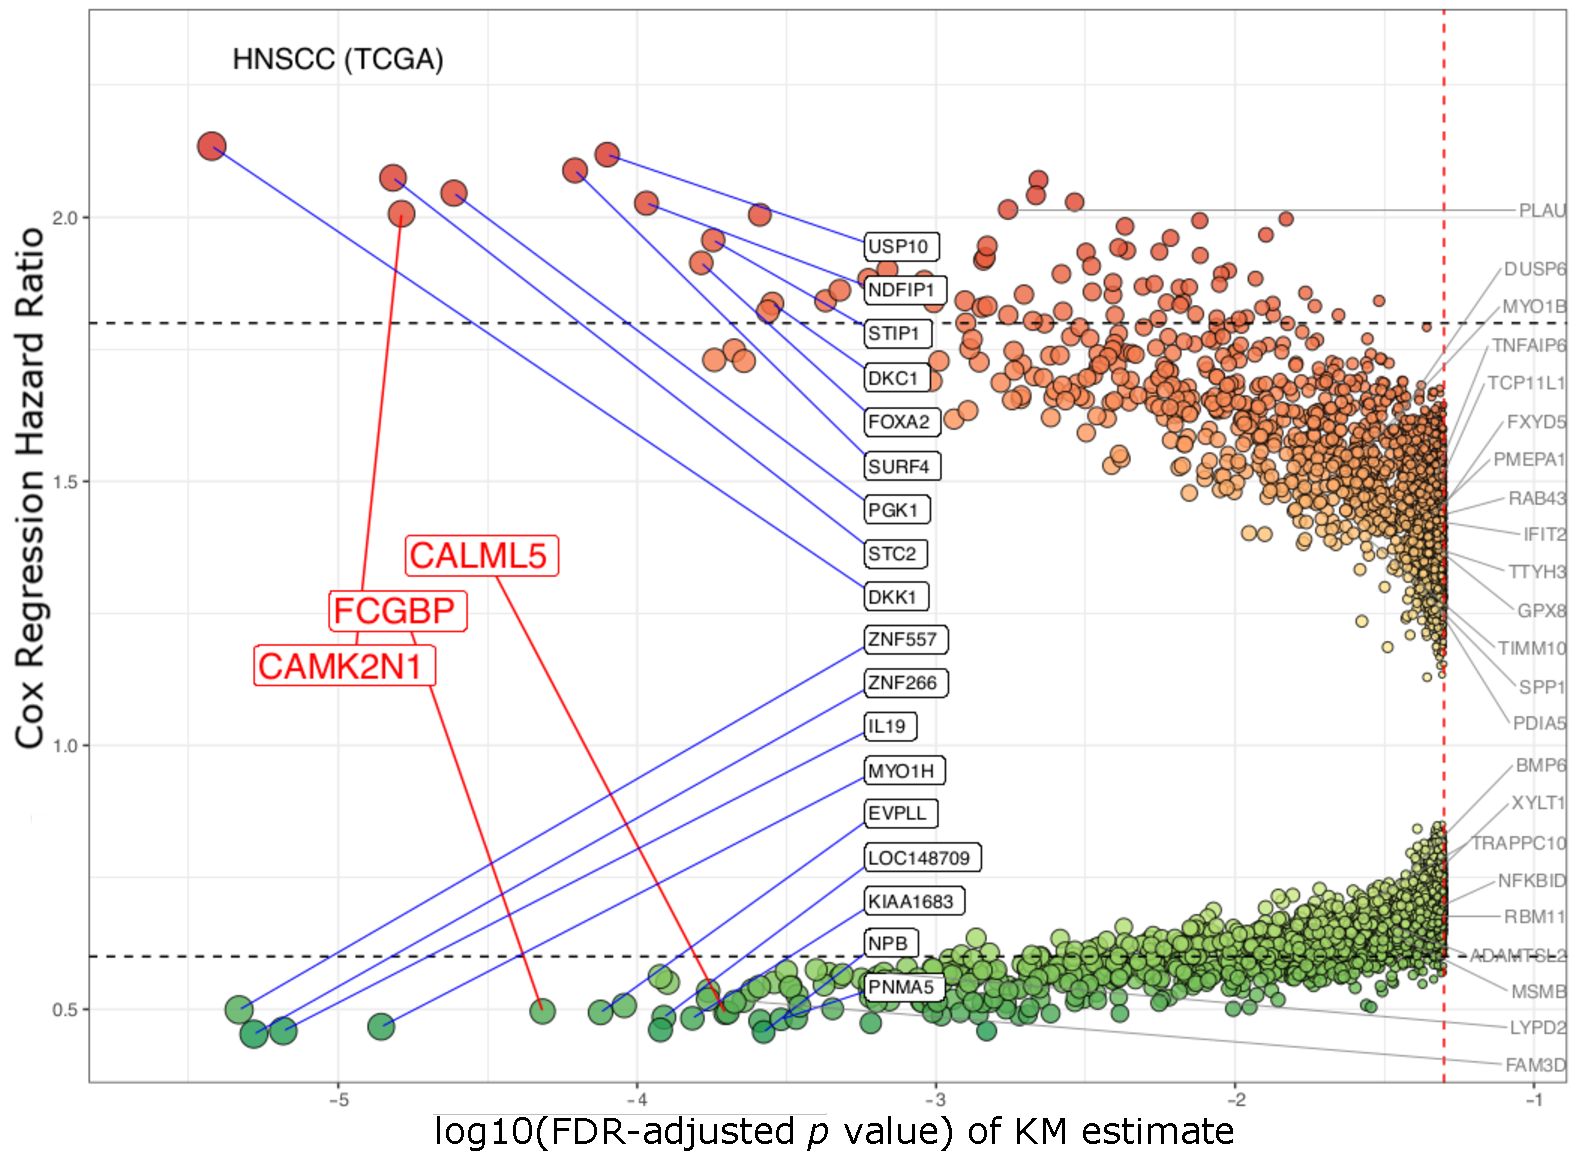
\includegraphics[width=13cm]{Rplot_TCGA_HNSCC_CoxHR_CAMK2N1_top3FDRKM.pdf}}
{    \caption{A volcano plot of genes in survival analyses of TCGA HNSCC.
%X axis: unadjusted \protect\textit{p}~value of Kaplan--Meier survival (-log10 transformed).
%Y axis: multivariate hazard ratio from Cox proportional regression model.
%Dotted line: significant Bonferroni corrected \protect\textit{p}~value. 
%\textcolor{red}{Red dots} mark 10 genes (unvalidated), which impact on poor prognosis ($HR>=1.5$). \textcolor{green}{Green dots} mark 10 genes (unvalidated), which affect on better survival ($HR<=0.5$).
    This cohort was applied for exploration of the candidate biomarkers.
    A total of 9416 genes had %\acrshort{fdr}-
    unadjusted \protect\textit{p}~values of less than 0.05.
    \textcolor{red}{CAMK2N1}, \textcolor{red}{CALML5}, \textcolor{red}{FCGBP}, and 17 other genes (marked in \textcolor{black}{black square}) had hazard ratios (HRs) >$1.8$ or <$0.6$.
    The 22 genes, listed on the side, had hazard ratios between 0.6 and 1.5.
    \textcolor{red}{Red spots}: $HR$ > 1.0.
    \textcolor{green}{Green spots}: $HR$ < 1.0.
    (X-axis: Kaplan--Meier survival estimates, with \acrshort{fdr}-adjusted \protect\textit{p}~values (log10 transformed);
y-axis: HR of Cox proportional hazard regression model.)
    }}
%%%\label{fig:hazards3}
\end{figure}

\begin{figure}[ht]

\floatbox[{\capbeside\thisfloatsetup{capbesideposition={right,center},capbesidewidth=.35\linewidth,capbesidesep=quad}}]{figure}[\FBwidth]
   % \centering
{    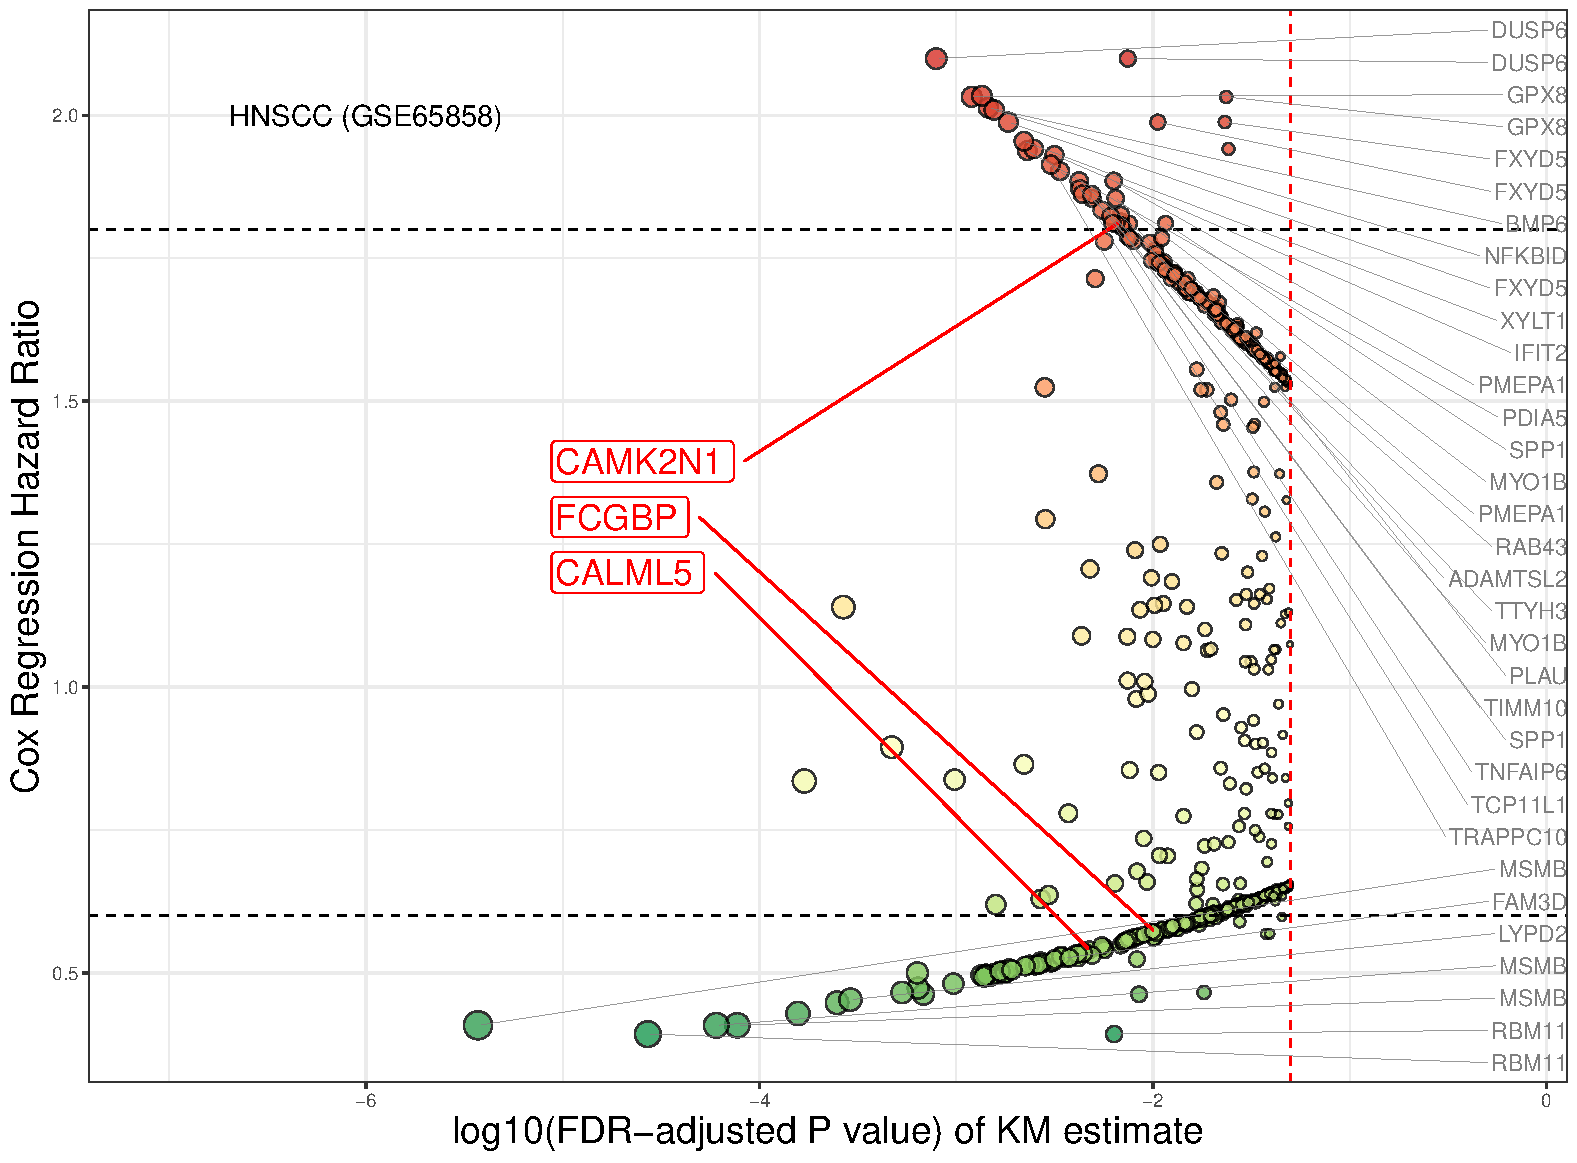
\includegraphics[width=13cm]{Rplot_GSE65858_CoxHR_CAMK2N1_top3FDRKM.pdf}}
{    \caption{Volcano plot of genes in survival analyses of GSE65858 cohort.
    % GSE117973 using the same platform GPL10558
    This HNSCC cohort was used for filtering of our candidate genes: \textcolor{red}{CAMK2N1}, \textcolor{red}{CALML5}, and \textcolor{red}{FCGBP}.
    In total, 534 genes had \acrshort{fdr}-adjusted \protect\textit{p}~values less than 0.05
    \textcolor{red}{Red spots}: hazard ratios are greater than 1.0;
    \textcolor{green}{Green spots}: hazard ratios are under 1.0.
    The 22 genes, listed on the side, had hazard ratios >$1.8$ or <$0.6$.
    (X-axis: Kaplan--Meier survival estimates, with \acrshort{fdr}-adjusted \protect\textit{p}~values, log10 transformed; y-axis: the hazard ratio (HR) under the Cox proportional hazard regression model).
    }}
%%%\label{fig:hazards534}
\end{figure}

\begin{figure}[ht]

\floatbox[{\capbeside\thisfloatsetup{capbesideposition={right,center},capbesidewidth=.35\linewidth,capbesidesep=quad}}]{figure}[\FBwidth]
% TCGA FDR Pvalue of CAMK2N1 (1.628308e-05), IL19 ( 6.543871e-06), FCGBP (4.827833e-05), CALML5 (0.0001970348)
{\setlength{\unitlength}{.78cm}
\begin{picture}(15, 20) %(1,0.55038404)%
\centering
  \put(0,0){\includegraphics[width=14cm]{Figure_4_CAMK2N1_CALML5_FCGBP.pdf}}%
  \put(2.5, 15.3){\fontfamily{qcr}\selectfont
  \tiny *\protect\textit{p} = \num{1.63e-05}}%CAMK2N1
    \put(2.5, 9.25){\fontfamily{qcr}\selectfont
  \tiny *\protect\textit{p} = \num{1.97e-4}}%IL19 6.54e-06 -> CALML5 0.0001970348
    \put(2.5, 2.45){\fontfamily{qcr}\selectfont
  \tiny *\protect\textit{p} = \num{4.83e-05}}%FCGBP

%\begin{annotationimage}{width=15cm}{Figure_4_CAMK2N1_IL19_FCGBP.pdf}
%\includegraphics[width=15cm]{Figure_4_CAMK2N1_IL19.pdf}
%\draw[annotation left = {Aries at 0.3}]

%\end{annotationimage}
\end{picture}%
}

{\caption{Kaplan--Meier survival analyses, by cutoff finding.
The Kaplan--Meier curves of (\textbf{a}) CAMK2N1, (\textbf{c}) CALML5, and (\textbf{e}) FCGBP with optimal \protect\textit{p}~values. 
%((b) the cutoffs derived from it's cumulative \protect\textit{p}~value plot).
%(c) Kaplan--Meier plot of IL19 under optimal \protect\textit{p}~value;
%((d) the cutoffs derived from it's cumulative \protect\textit{p}~value plot).
%(e) Kaplan--Meier plot of FCGBP under optimal \protect\textit{p}~value.\\
%The optimal cutoff value for CAMK2N1 is 
The cutoffs in the cumulative \protect\textit{p}~value plots of (\textbf{b}) CAMK2N1, (\textbf{d}) CALML5, and (\textbf{f}) FCGBP,
show that over 50\% of those unadjusted \protect\textit{p}~values derived by the sliding-window cutoff-finding procedure are below 0.001.
(* \protect\textit{p}: \protect\textit{p}~value adjusted by \acrlong{fdr}, \acrshort{fdr}.)
}}
%%%\label{fig:figure4}
\end{figure}

\begin{table}[H] 
%\centering
%%%\caption{Univariate/multivariate Cox proportional hazard regression analyses on OS time of CAMK2N1 gene expression in HNSCC.}

%%%\label{table:table2}
\arrayrulecolor[rgb]{0.255,0.255,0.255}


\resizebox{\linewidth}{!}{%
\begin{tabular}{|l|l|c|c|c|c|c|c|} 
\noalign{\hrule height 1.0pt}
%\begin{tabularx}{\textwidth}{|p{2.5cm}|l|l|l|l|l|l|l|} 
%\arrayrulecolor{black}\cline{1-2}
\arrayrulecolor[rgb]{0.255,0.255,0.255}
\cline{3-8}
\multicolumn{2}{|l!{\color{black}\vrule}}{\multirow{2}{*}{\textbf{Features}}}                                                          & \multicolumn{3}{c|}{\textbf{Univariate}}                                                                                                                                                                                                                & \multicolumn{3}{c|}{\textbf{Multivariate}}                                                                                                                                                                                                               \\ 
\cline{3-8}
\multicolumn{2}{|l!{\color{black}\vrule}}{}                                                                                   & \multicolumn{1}{l!{\color{black}\vrule}}{\textbf{HR}}                                   & \multicolumn{1}{c!{\color{black}\vrule}}{\textbf{CI95\%}}                              & \multicolumn{1}{l!{\color{black}\vrule}}{\textbf{\protect\textit{p}~Value}}                    & \multicolumn{1}{l!{\color{black}\vrule}}{\textbf{HR}}                                   & \multicolumn{1}{c!{\color{black}\vrule}}{\textbf{CI95\%}}                              & \multicolumn{1}{l!{\color{black}\vrule}}{\textbf{\protect\textit{p}~Value}}                     \\ 
\arrayrulecolor{black}\hline
\multirow{2}{*}{Gender}                 & \multicolumn{1}{l!{\color{black}\vrule}}{{\cellcolor[rgb]{0.62,0.812,0.878}}Female} & \multicolumn{1}{l!{\color{black}\vrule}}{{\cellcolor[rgb]{0.62,0.812,0.878}}1} & \multicolumn{1}{l!{\color{black}\vrule}}{{\cellcolor[rgb]{0.62,0.812,0.878}}} & \multicolumn{1}{l!{\color{black}\vrule}}{{\cellcolor[rgb]{0.62,0.812,0.878}}} & \multicolumn{1}{l!{\color{black}\vrule}}{{\cellcolor[rgb]{0.62,0.812,0.878}}1} & \multicolumn{1}{l!{\color{black}\vrule}}{{\cellcolor[rgb]{0.62,0.812,0.878}}} & \multicolumn{1}{l!{\color{black}\vrule}}{{\cellcolor[rgb]{0.62,0.812,0.878}}}  \\ 
\cline{2-8}
                                        & Male                                                                                & 1.157                                                                          & 0.843--1.587                                                                   & 0.367                                                                         & 1.076                                                                          & 0.767--1.510                                                                   & 0.671                                                                          \\ 
\arrayrulecolor[rgb]{0.255,0.255,0.255}\hline
\multirow{2}{*}{Age at diagnosis}       & {\cellcolor[rgb]{0.62,0.812,0.878}}$<=65y$                                             & {\cellcolor[rgb]{0.62,0.812,0.878}}1                                           & {\cellcolor[rgb]{0.62,0.812,0.878}}                                           & {\cellcolor[rgb]{0.62,0.812,0.878}}                                           & {\cellcolor[rgb]{0.62,0.812,0.878}}1                                           & {\cellcolor[rgb]{0.62,0.812,0.878}}                                           & {\cellcolor[rgb]{0.62,0.812,0.878}}                                            \\ 
\cline{2-8}
                                        & $>65y$                                                                                 & 1.329                                                                          & 0.990--1.784                                                                   & 0.058                                                                         & 1.391                                                                          & 1.025--1.888                                                                   & \textcolor{red}{0.034}                                                         \\ 
\hline
\multirow{2}{*}{Clinical T Status}      & {\cellcolor[rgb]{0.62,0.812,0.878}}T1+T2                                            & {\cellcolor[rgb]{0.62,0.812,0.878}}1                                           & {\cellcolor[rgb]{0.62,0.812,0.878}}                                           & {\cellcolor[rgb]{0.62,0.812,0.878}}                                           & {\cellcolor[rgb]{0.62,0.812,0.878}}1                                           & {\cellcolor[rgb]{0.62,0.812,0.878}}                                           & {\cellcolor[rgb]{0.62,0.812,0.878}}                                            \\ 
\cline{2-8}
                                        & T3+T4                                                                               & 1.409                                                                          & 1.028--1.931                                                                   & \textcolor{red}{0.033}                                                        & 1.982                                                                          & 1.048--3.745                                                                   & \textcolor{red}{0.035}                                                         \\ 
\hline
\multirow{2}{*}{Clinical N Status}      & {\cellcolor[rgb]{0.62,0.812,0.878}}N0                                               & {\cellcolor[rgb]{0.62,0.812,0.878}}1                                           & {\cellcolor[rgb]{0.62,0.812,0.878}}                                           & {\cellcolor[rgb]{0.62,0.812,0.878}}                                           & {\cellcolor[rgb]{0.62,0.812,0.878}}1                                           & {\cellcolor[rgb]{0.62,0.812,0.878}}                                           & {\cellcolor[rgb]{0.62,0.812,0.878}}                                            \\ 
\cline{2-8}
                                        & N1-3                                                                                & 1.185                                                                          & 0.890--1.577                                                                   & 0.246                                                                         & 1.145                                                                          & 0.801--1.636                                                                   & 0.457                                                                          \\ 
\hline
\multirow{2}{*}{Clinical M Status}      & {\cellcolor[rgb]{0.62,0.812,0.878}}M0                                               & {\cellcolor[rgb]{0.62,0.812,0.878}}1                                           & {\cellcolor[rgb]{0.62,0.812,0.878}}                                           & {\cellcolor[rgb]{0.62,0.812,0.878}}                                           & {\cellcolor[rgb]{0.62,0.812,0.878}}1                                           & {\cellcolor[rgb]{0.62,0.812,0.878}}                                           & {\cellcolor[rgb]{0.62,0.812,0.878}}                                            \\ 
\cline{2-8}
                                        & M1                                                                                  & 4.097                                                                          & 1.009--16.644                                                                  & \textcolor{red}{0.049}                                                        & 7.314                                                                          & 1.590--33.631                                                                  & \textcolor{red}{0.011}                                                         \\ 
\hline
\multirow{2}{*}{Clinical Stage}         & {\cellcolor[rgb]{0.62,0.812,0.878}}Stage I+II                                       & {\cellcolor[rgb]{0.62,0.812,0.878}}1                                           & {\cellcolor[rgb]{0.62,0.812,0.878}}                                           & {\cellcolor[rgb]{0.62,0.812,0.878}}                                           & {\cellcolor[rgb]{0.62,0.812,0.878}}1                                           & {\cellcolor[rgb]{0.62,0.812,0.878}}                                           & {\cellcolor[rgb]{0.62,0.812,0.878}}                                            \\ 
\cline{2-8}
                                        & Stage III+IV                                                                        & 1.245                                                                          & 0.882--1.759                                                                   & 0.213                                                                         & 0.621                                                                          & 0.287--1.343                                                                   & 0.226                                                                          \\ 
\hline
\multirow{2}{*}{Surgical Margin status} & {\cellcolor[rgb]{0.62,0.812,0.878}}Negative                                         & {\cellcolor[rgb]{0.62,0.812,0.878}}1                                           & {\cellcolor[rgb]{0.62,0.812,0.878}}                                           & {\cellcolor[rgb]{0.62,0.812,0.878}}                                           & {\cellcolor[rgb]{0.62,0.812,0.878}}1                                           & {\cellcolor[rgb]{0.62,0.812,0.878}}                                           & {\cellcolor[rgb]{0.62,0.812,0.878}}                                            \\ 
\cline{2-8}
                                        & Positive                                                                            & 1.591                                                                          & 1.155--2.191                                                                   & \textcolor{red}{0.004}                                                        & 1.631                                                                          & 1.182--2.250                                                                   & \textcolor{red}{0.003}                                                         \\ 
\hline
\multirow{2}{*}{Tobacco Exposure}       & {\cellcolor[rgb]{0.62,0.812,0.878}}Low                                              & {\cellcolor[rgb]{0.62,0.812,0.878}}1                                           & {\cellcolor[rgb]{0.62,0.812,0.878}}                                           & {\cellcolor[rgb]{0.62,0.812,0.878}}                                           & {\cellcolor[rgb]{0.62,0.812,0.878}}1                                           & {\cellcolor[rgb]{0.62,0.812,0.878}}                                           & {\cellcolor[rgb]{0.62,0.812,0.878}}                                            \\ 
\cline{2-8}
                                        & High                                                                                & 1.364                                                                          & 1.008--1.844                                                                   & \textcolor{red}{0.044}                                                        & 1.363                                                                          & 0.990--1.875                                                                   & 0.058                                                                          \\ 
\hline
\multirow{2}{*}{Gene Expression}                & {\cellcolor[rgb]{0.62,0.812,0.878}}Low                                              & {\cellcolor[rgb]{0.62,0.812,0.878}}1                                           & {\cellcolor[rgb]{0.62,0.812,0.878}}                                           & {\cellcolor[rgb]{0.62,0.812,0.878}}                                           & {\cellcolor[rgb]{0.62,0.812,0.878}}1                                           & {\cellcolor[rgb]{0.62,0.812,0.878}}                                           & {\cellcolor[rgb]{0.62,0.812,0.878}}                                            \\ 
\cline{2-8}
                                        & High                                                                                & 2.101                                                                          & 1.572--2.809                                                                   & \multicolumn{1}{c|}{\textcolor{red}{\textless{} 0.001}}                                     & 2.007                                                                          & 1.490--2.704                                                                   & \multicolumn{1}{c|}{\textcolor{red}{\textless{} 0.001}}                                      \\ 
%\hline
%\multicolumn{8}{|l|}{}                                                                                                                                                                                                                                                                                                                                                                                                                                                                                                                                                                                                           \\ 
%\hline
% \\
\noalign{\hrule height 1.0pt}
\end{tabular}
} % end of \resizebox

\pbox{\columnwidth}{\footnotesize {
(OS: overall survival;
HR: hazard ratio;
CI95\%: 95\% confidence interval;
\protect\textit{p}~value significant code is denoted: red \textless{} 0.05).} %; *** \textless{} 0.001).}                                        
}
%\arrayrulecolor{black}
\end{table}

\begin{table}[H] 
%\centering
%%%\caption{The top 3 genes with prognostic impacts on HNSCC.}% (ranked by Bonferroni-adjusted \protect\textit{p}~values}

%%%\label{tab:newTable1}
\resizebox{\linewidth}{!}{% \textwidth
\begin{tabular}{|l|l|l|c|c|c|c|c|c|}
\noalign{\hrule height 1.0pt}
\multicolumn{1}{|c|}{} &
  \multicolumn{2}{c|}{} &
  \multicolumn{2}{c|}{\textbf{Kaplan--Meier Survival}} &
  \multicolumn{2}{c|}{\textbf{Cox Univariate}} &
  \multicolumn{2}{c|}{\textbf{Cox Multivariate}} \\ \cline{4-9} 
\multicolumn{1}{|l|}{\multirow{-2}{*}{\textbf{Gene ID}}} &
  \multicolumn{2}{l|}{\multirow{-2}{*}{\textbf{Gene Descriptio}n}} &
  \begin{tabular}[c]{@{}c@{}}\textbf{FDR}\\ \textbf{\protect\textit{p}~Value}\end{tabular} &
  \begin{tabular}[c]{@{}c@{}}\textbf{Bonferroni}\\ \textbf{\protect\textit{p}~Value}\end{tabular} &
  \textbf{HR *} &
  \textbf{CI95\%} &
  \textbf{HR *} &
  \textbf{CI95\%} \\ 
  \hline
CAMK2N1 &
  \multicolumn{2}{l|}{\begin{tabular}[c]{@{}l@{}}calcium/calmodulin-\\ dependent protein\\ kinase II inhibitor 1\end{tabular}} &
  \num{1.63e-5} & %2.9e-7} &
  0.002 &
  2.101 &
  1.572--2.809 &
  2.007 &
  1.490--2.704 \\ \hline
CALML5 &
  \multicolumn{2}{l|} {\acrlong{CALML5}} &
   \num{1.97e-4} & %\num{6.54e-6} & %3.7e-7} &
   0.039 &
   0.51 &
   0.379--0.686 &
   0.493 &
   0.364--0.667 \\ \hline
FCGBP &
  \multicolumn{2}{l|}{\begin{tabular}[c]{@{}l@{}}Fc fragment of\\  IgG binding protein\end{tabular}} &
   \num{4.83e-5} & %1.2e-6} &
   0.008 &
   0.484 &
   0.359--0.653 &
   0.496 &
   0.366--0.674 \\ 
\noalign{\hrule height 1.0pt}
%\multicolumn{9}{|l|}{} \\
%\multicolumn{9}{|l|}%{\multirow{-0}{*}
%{\begin{tabular}[c]{@{}l@{}}
%
%\end{tabular}
%%}\\ % within \multirow
%} \\ % within \multicolumn
%\hline
%\multicolumn{9}{|l|}{ \\ \hline

\end{tabular}%
}
\pbox{\columnwidth}{\footnotesize Selection criteria (fit all): 
(1) Kaplan--Meier Bonferroni-adjusted \protect\textit{p} \textless~0.05; 
(2) Cox's univariate and multivariate HR \textgreater{}= 1.8 or \textless{}= 0.6 in TCGA cohort; 
(3) Cox's univariate and multivariate HR \textgreater{}= 1.8 or \textless{}= 0.6 in GSE65858 cohort.\\
*~Cox's model: \protect\textit{p} \textless 0.001
(HR: hazard ratio; CI95\%: 95\% confidence interval; FDR: \acrlong{fdr}).}

\end{table}


\section{Discussion}


\subsection{The Three Biomarkers in Cancer}


\subsubsection{The Protein/Pathology Atlas} %still TCGA's RNA-Seq (ok)


\subsubsection{Literature Review} % literature (ok)


\subsection{Feature Selection for Survival Modeling} % Even there are many $X_1 ... X_n$ physical and social features of patients available for survival modelling in the TCGA.


\subsection{The Purpose of Sliding-Window Cutoff Selection}


\subsection{Technical Considerations}


\subsection{Limitations of the Study}

\begin{figure}[ht]

\floatbox[{\capbeside\thisfloatsetup{capbesideposition={right,center},capbesidewidth=.35\linewidth,capbesidesep=quad}}]{figure}[\FBwidth]
{%\widefigure
    %\centering
    
    \begin{subfigure}[a]{0.5\textwidth}
    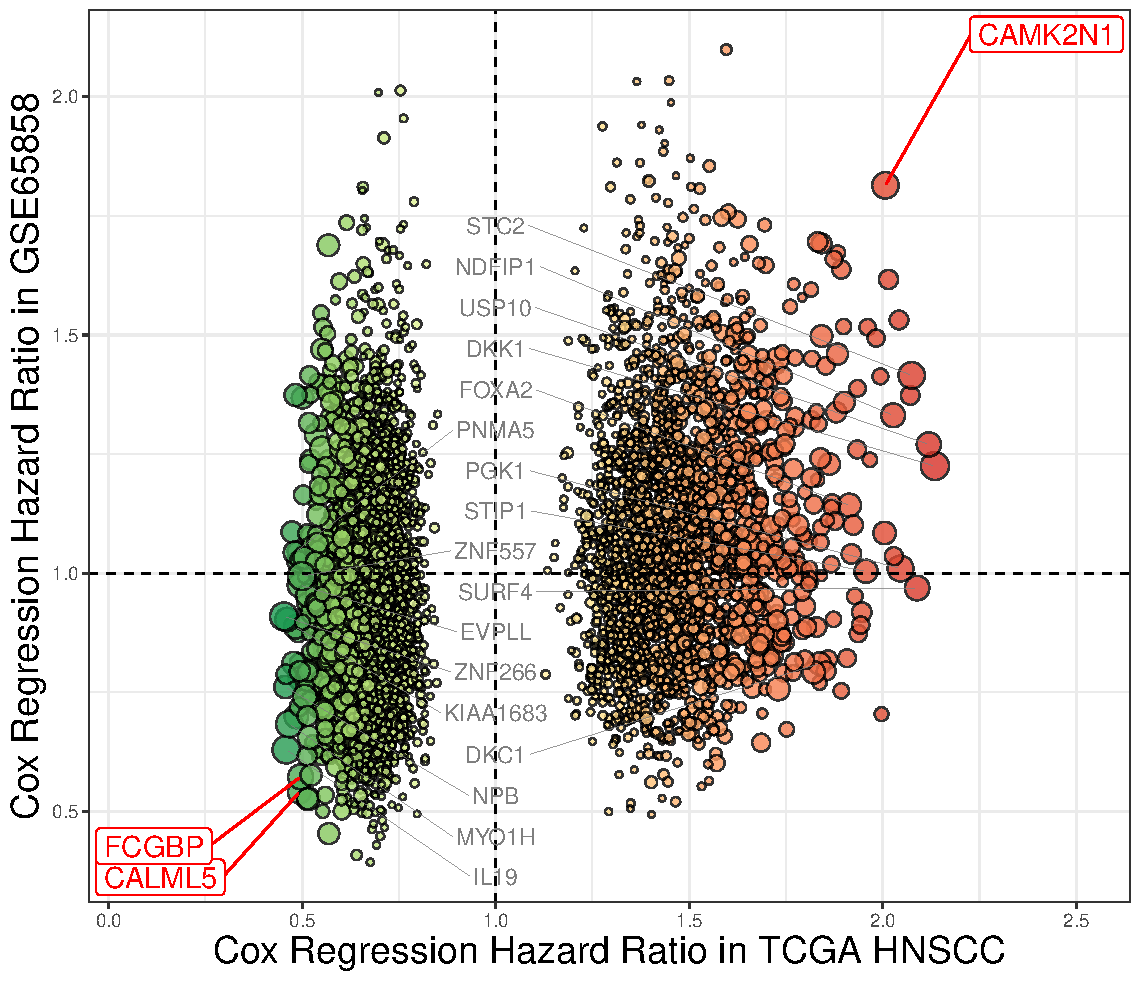
\includegraphics[width=9cm]{RplotH2H_TCGA_GSE65858_CoxHR.pdf}
    \caption{Cox's hazard ratios from TCGA HNSCC and GSE65858 (Pearson's correlation coefficient~\cite{Schober2018}, r = 0.27).}
    \end{subfigure}
%\hfill
    \begin{subfigure}[b]{0.2\textwidth}
    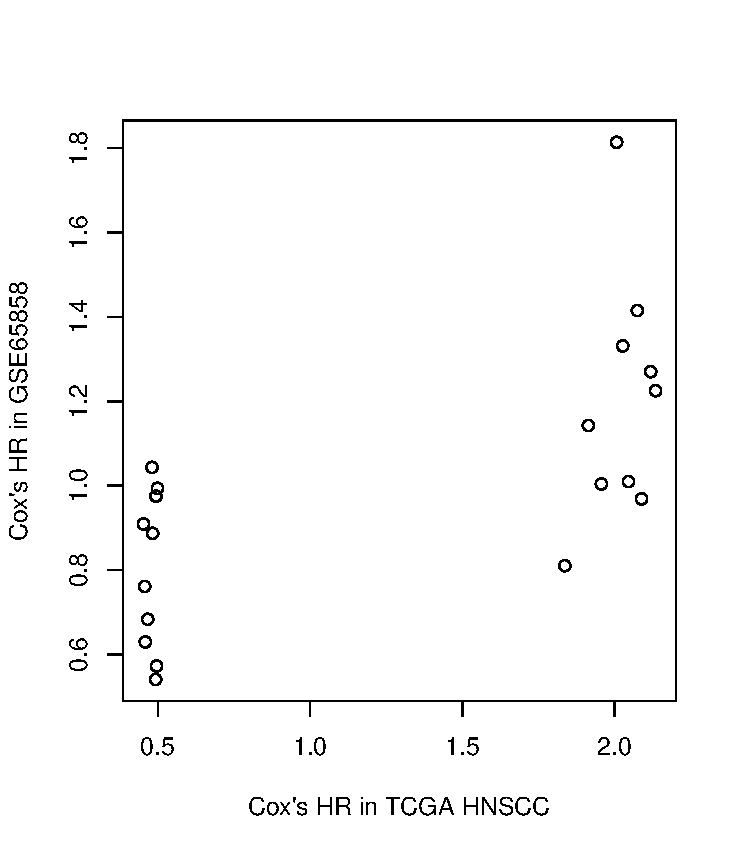
\includegraphics[width=3cm]{Rplot20_correlation_TCGA_GSE65858_CoxHR.pdf}
    \caption{Correlations of Cox's hazard ratios of those 20 significant genes (Pearson's r = 0.68).}
    \end{subfigure}    
}   
{    \caption{A head-to-head comparison of Cox's hazard ratios from TCGA HNSCC and GSE65858 datasets.
TCGA HNSCC and GSE65858 cohorts were applied for identification and validation of the candidate biomarkers in HNSCC.
    (\textbf{a}) A total of 5404 genes had Cox's hazard ratios from TCGA HNSCC and GSE65858 (Pearson's correlation, r = 0.27).
    %\acrshort{fdr}-\protect\textit{p}~values of less than 0.05 in TCGA HNSCC.
    \textcolor{red}{CAMK2N1}, \textcolor{red}{CALML5}, \textcolor{red}{FCGBP}, and 17 other genes (marked in \textcolor{black}{black}) had hazard ratios (HRs) >$1.8$ or <$0.6$.
    \textcolor{red}{Red spots}: $HR$s > 1.0 in TCGA HNSCC.
    \textcolor{green}{Green spots}: $HR$s < 1.0 in TCGA HNSCC.
    Sizes of spots: bigger for Kaplan--Meier \protect\textit{p}~values in TCGA HNSCC. %Please ensure intended meaning is retained.
    (\textbf{b}) The 20 genes were extracted and shown. The hazard ratios of those genes have a moderate correlation between the two cohorts (Pearson's r = 0.68).
    (X-axis: Hazard ratios of Cox proportional hazard regression model from TCGA HNSCC;
    y-axis: Those values from GSE65858; TCGA: \acrlong{tcga}; HNSCC: \acrlong{hnscc}.)
    }}
%%%\label{fig:hazards_head2head_TCGA_GSE65858}
\end{figure}


\subsection{Future Directions in Translational Medicine}


\subsubsection{Proteomics Validation}


\subsubsection{Laboratory Validation}


\subsubsection{Cancer Type-Agnostic Study}


\subsubsection{Holistic Cancer Care} 

\begin{figure}[ht]

\floatbox[{\capbeside\thisfloatsetup{capbesideposition={right,center},capbesidewidth=.35\linewidth,capbesidesep=quad}}]{figure}[\FBwidth]
\centering

{\setlength{\unitlength}{.78cm}
\begin{picture}(15, 20) %(1,0.55038404)%
\centering
  \put(0,0){\includegraphics[width=11cm]{Figure_5_holisticCare.pdf}}%
  \put(1.4, 6.9){\fontfamily{qcr}\selectfont
  \tiny \textbf{[Physician]}}%

%\includegraphics[width=10cm]{Figure_5_holisticCare.pdf}
\end{picture}
}
{\caption{The concept of holistic care for \acrshort{hnscc} patients. %MDPI: please confirm if the extra lines and frame need to be deleted.
Beyond carcinogenesis: In the mind--brain--body axis, a stressful environment (giant \textcolor{black}{black} arrow) will trigger an emotional response. The subconscious mind (brain) releases stress hormones and inflammation signals in response to negative emotions. The  body's internal environment (cells) alters epigenetic control in gene regulation and mRNA expression. Over a long time, the tissue/cells will be transformed into dysplasia and then malignancy (e.g., HNSCC) with help from known carcinogens.
Cancer care: Holistic care should take care of cancer patients' spiritual, emotional, physical, and socioeconomic needs. Physical care will be carried out by medication therapy or surgery. After establishing a therapeutic relationship (TR), the physicians' spiritual properties (empathy, sympathy, and compassion) will engage cancer patients and recover their self-compassion to gain resilience against the disease through their mind--brain--body axis.
Thus, we suggest that electric healthcare records (EHR) should include physical, pathological, and psychological data, and even more spiritual information. The \acrshort{tcga} might collect those "holistic features"  (\textcolor{green}{green} dashed line) for further study of personalized medicine.}
}

%%%\label{fig:figure5}
\end{figure}


\section{Materials and Methods} % 4


\subsection{Patient Cohort} 


\subsubsection{RNA Sequencing Data} 


\subsubsection{Clinical Data} 


\subsection{Cutoff Finder Core Engine}


\subsection{Statistical Consideration for Survival Analysis}


\subsection{Biomarker Selection and Validation}


\section{Conclusions} % 5



%%%%%%%%%%%%%%%%%%%%%%%%%%%%%%%%%%%%%%%%%%%%%%%%%%%%%%%%%%%%%%%
\clearpage
%%%%%%%
\thispagestyle{empty} % No slide header and footer

\bibliographystyle{unsrt}
\bibliography{sample}

\clearpage

%------------------------------------------------

\thispagestyle{empty} % No slide header and footer

\begin{tikzpicture}[remember picture,overlay] % Background box
  \node [xshift=\paperwidth/2,yshift=\paperheight/2] at (current page.south west)
    [rectangle,fill,inner sep=0pt,minimum width=\paperwidth,minimum height=\paperheight/2.1,top color=myblue,bottom color=myblue]{}; % Change the height of the box, its colors and position on the page here
\end{tikzpicture}
% Text within the box
\begin{flushright}
  \vspace{1.6cm}
  \color{white}\sffamily
  {\bfseries\Large Comments and Suggestions\par}% Title
  \vspace{0.5cm}
  \normalsize
%  \myauthor\par % Author name
%  \mydate\par % Date
  \myuni\par
  \vfill
\end{flushright}

%----------------------------------------------------------------------------------------
%
\end{document}